\documentclass{article}
\usepackage{titlesec}
%Referencias
\usepackage[style=authortitle,backend=bibtex]{biblatex}
\addbibresource{functional-analysis.bib}

%Paquetes
\usepackage[left=4cm, right=4cm]{geometry}
\usepackage{palatino}%Fuente
\usepackage{graphicx}%Imágenes
\usepackage{float}%Imágenes
\usepackage{subcaption}%Imágenes
\usepackage{enumitem}%Listas
\usepackage{parskip}%Espacio entre párrafos
\usepackage{multicol}
\usepackage{amsthm,thmtools,xcolor}
\usepackage{amssymb}%Mate
\usepackage{amsmath}%Mate
\usepackage{tikz}%Mate (diagramas)
\usepackage{dutchcal}
\usepackage{tikz-cd}
\usepackage{xcolor}
\definecolor{blue-violet}{rgb}{0.54, 0.17, 0.89}
\usetikzlibrary{%
	matrix,%
	calc,%
	arrows,%
	shapes,
	decorations.markings,backgrounds,calc,intersections
}
\usepackage[bookmarks,bookmarksopen,bookmarksdepth=3]{hyperref}%Links a lugares en el texto
\hypersetup{%colores
	colorlinks=true,
	urlcolor=blue,
	linkcolor=magenta,
	citecolor=blue,
	filecolor=blue,
	urlbordercolor=white,
	linkbordercolor=white,
	citebordercolor=white,
	filebordercolor=white
}
\usepackage{cleveref}


%Referencias
%\usepackage[style=authortitle,backend=bibtex]{biblatex}
%\addbibresource{analysis.bib}

\definecolor{blue-violet}{rgb}{0.54, 0.17, 0.89}
\definecolor{azure}{rgb}{0.0, 0.5, 1.0}
\definecolor{green(ncs)}{rgb}{0.0, 0.62, 0.42}
\definecolor{forestgreen}{rgb}{0.13, 0.55, 0.13}
\definecolor{limegreen}{rgb}{0.2, 0.8, 0.2}
\definecolor{palatinateblue}{rgb}{0.15, 0.23, 0.89}
\definecolor{trueblue}{rgb}{0.0, 0.45, 0.81}
\definecolor{goldenyellow}{rgb}{1.0, 0.87, 0.0}
\definecolor{fashionfuchsia}{rgb}{0.96, 0.0, 0.63}
\definecolor{brightcerulean}{rgb}{0.11, 0.67, 0.84}
\definecolor{jonquil}{rgb}{0.98, 0.85, 0.37}
\definecolor{lavendermagenta}{rgb}{0.93, 0.51, 0.93}
\definecolor{peru}{rgb}{0.8, 0.52, 0.25}
\definecolor{persimmon}{rgb}{0.93, 0.35, 0.0}
\definecolor{persianred}{rgb}{0.8, 0.2, 0.2}
\definecolor{persianblue}{rgb}{0.11, 0.22, 0.73}
\definecolor{persiangreen}{rgb}{0.0, 0.65, 0.58}
\definecolor{persianyellow}{rgb}{0.9, 0.89, 0.0}

\theoremstyle{definition}
\newtheorem{theorem}{Theorem}[section]

\declaretheoremstyle[headfont=\color{trueblue}\normalfont\bfseries
%bodyfont=\color{trueblue}
\normalfont,]{colored1}
\declaretheoremstyle[headfont=\color{forestgreen}\normalfont\bfseries,]{colored2}
\declaretheoremstyle[headfont=\color{peru}\normalfont\bfseries,]{colored3}
\declaretheoremstyle[headfont=\color{persiangreen}\normalfont\bfseries,]{colored4}
\declaretheoremstyle[headfont=\color{brightcerulean}\normalfont\bfseries,]{colored5}
\declaretheoremstyle[headfont=\color{lavendermagenta}\normalfont\bfseries,]{colored6}
\declaretheoremstyle[headfont=\color{blue-violet}\normalfont\bfseries,]{colored7}
\declaretheoremstyle[headfont=\color{green(ncs)}\normalfont\bfseries,]{colored8}

\declaretheorem[style=colored1,numberwithin=section,name=Theorem]{thm}
\declaretheorem[style=colored2,numberwithin=section,numberlike=thm,name=Proposition]{prop}
\declaretheorem[style=colored3,numberwithin=section,numberlike=thm,name=Lemma]{lemma}
\declaretheorem[style=colored4,numberwithin=section,numberlike=thm,name=Corollary]{coro}
\declaretheorem[style=colored5,numbered=no,name=Example]{example}
\declaretheorem[style=colored5,numbered=no,name=Examples]{examples}
\declaretheorem[style=colored6,numberwithin=section,name=Exercise]{exer}
\declaretheorem[style=colored6,numbered=no,name=Exercise]{exer*}
\declaretheorem[style=colored7,numberwithin=section,name=Remark]{remark}
\declaretheorem[style=colored8,numberwithin=section,name=Claim]{claim}

\numberwithin{equation}{section}


\newtheorem*{defn}{Definition}
\newtheorem*{question}{question}

\newcommand{\R}{\mathbb{R}}
\newcommand{\Z}{\mathbb{Z}}
\newcommand{\N}{\mathbb{N}}
\newcommand{\C}{\mathbb{C}}
\newcommand{\Q}{\mathbb{Q}}
\newcommand{\D}{\mathbb{D}}
\newcommand{\Cinf}{C^\infty}

\DeclareMathOperator{\img}{img}
\DeclareMathOperator{\Arg}{Arg}
\DeclareMathOperator{\Id}{Id}
\DeclareMathOperator{\Alt}{Alt}
\DeclareMathOperator{\sgn}{sgn}
\DeclareMathOperator{\supp}{supp}
\DeclareMathOperator{\Int}{Int}

\begin{document}
	\begin{center}
		{\LARGE Functional Analysis}

		\href{https://github.com/dan-gc/analysis}{github.com/dan-gc/analysis}
	\end{center}
	These are preparation notes for a course on Functional Analysis at IMPA, summer 2024. They are based on \cite{folland,narici,brezis}.
	\tableofcontents
	\clearpage
\section{Measure theory}
	{\small \color{blue}A measure should surely satisfy:
	\begin{enumerate}
		\item If $E_1,E_2,\ldots$ is a finite or infinite sequence of disjoint sets,
		\[\mu(E_1\cup E_2\cup\ldots)=\mu(E_1)+\mu(E_2)+\ldots\]
		
		\item If $E$ is congruent to $F$,
		\[\mu(E)=\mu(F)\]
		
		\item If $Q$ is the unit cube,
		\[\mu(Q)=1\]
	\end{enumerate}}
	\subsection{$\sigma$-algebras}\label{subsec:sigma-algebras}
	Let $X$ be a nonempty set. 
	
	\begin{itemize}
	\item An \textbf{\textit{algebra of sets}} on $X$ is a nonempty collection $\mathcal{A}$ of subsets of $X$ that is closed under finite unions and complements, that is,
	\begin{enumerate}
		\item If $E_1,\ldots, E_n\in \mathcal{A}$, then $\bigcup_{i=1}^nE_i\in\mathcal{A}$.
		\item If $E\in\mathcal{A}$, then $E^c\in\mathcal{A}$.
	\end{enumerate}
	\item A \textbf{\textit{$\sigma$-algebra}} is an algebra of sets closed under countable unions.
		\item The intersection of all $\sigma$-algebras containing any subset $\mathcal{E}\subset \mathcal{P}(X)$ is the \textbf{\textit{$\sigma$-algebra generated by $\mathcal{E}$}}.
		
		\item The $\sigma$-algebra generated by the open sets of a topological (or metric) space $X$ is the \textbf{\textit{Borel algebra $\mathcal{B}_X$}}.
		
		\item Let $\{X_\alpha\}_{\alpha\in A}$ is a collection of nonempty sets, $X=\prod_\alpha X_\alpha$ and $\pi_\alpha:X\to X_\alpha$ the coordinate functions. If $\mathcal{M}_\alpha$ is a $\sigma$-algebra on $X_\alpha$, the \textbf{\textit{product $\sigma$-algebra}} on $X$ is the $\sigma$-algebra generated by
		\[\{\pi_\alpha(E_\alpha):E_\alpha\in\mathcal{M}_\alpha,\alpha\in A\}\]
		We denote this $\sigma$-algebra by $\bigotimes_{\alpha\in A}\mathcal{M}_\alpha$. 
		\begin{prop}
			$\bigotimes_{\alpha\in A}\mathcal{M}_\alpha$ is generated by $\{\prod_{\alpha\in A}E_\alpha:E_\alpha\in\mathcal{M}\}$. 
		\end{prop}
		\begin{prop}
			Let $X_1,\ldots,X_n$ be metric spaces and let $X=\prod_i X_i$ be equiped with the product metric. Then $\bigotimes_i\mathcal{B}_i\subset\mathcal{B}_X$. If every $X_i$ is separable equality holds.
		\end{prop}
		\begin{coro}
			$\mathcal{B}_{\R^n}=\bigotimes_{i=1}^n\mathcal{B}_{\R}$.
		\end{coro}
	\end{itemize}

	\subsection{Measures}
	%\item \textbf{(Measures.)}
	Let $X$ be a set equipped with a $\sigma$-algebra $\mathcal{M}$.
	\begin{itemize}
		\item A \textbf{\textit{measure}} on $\mathcal{M}$ (or on $(X,\mathcal{M})$, or simply on $X$) is a function $\mu:\mathcal{M}\to [0,\infty)$ such that
		\begin{enumerate}
			\item $\mu(\varnothing)$.
			\item if $\{E_j\}_{1}^\infty$ is a sequence of disjoint sets in $\mathcal{M}$, then $\mu\left(\bigcup_{1}^\infty\right)=\sum_1^\infty\mu(E_i)$.
		\end{enumerate}
		\item If $X$ is a set and $\mathcal{M}\subset\mathcal{P}(X)$ is a $\sigma$-algebra, $(X,\mathcal{M})$ is called a \textbf{\textit{measurable space}} and the sets in $\mathcal{M}$ are \textbf{\textit{measurable sets}}. If $\mu$ is a measure on $(X,\mathcal{M})$, then $(X,\mathcal{M},\mu)$ is called a \textbf{\textit{measure space}}.
		\item If $\mu(X)<\infty$ (and hence $\mu(E)<\infty$ for all $E\in\mathcal{M}$), $\mu$ is called \textbf{\textit{finite}}. If $X=\bigcup_{1}^\infty E_j$, with $\mu(E_j)<\infty$, $\mu$ is called \textbf{\textit{$\sigma$-finite}}. If for every $E\in\mathcal{M}$ with $\mu(E)=\infty$ there exists $F\in\mathcal{M}$ such that $F\subset E$ and $0<\mu(F)<\infty$, $\mu$ is called \textbf{\textit{semifinite}}.
		\begin{thm}[Properties of measure spaces]
			Let $(X,\mathcal{M},\mu)$ be a measure space.
			\begin{enumerate}
				\item \textbf{(Monotonicity.)} If $E,F\in\mathcal{M}$ and $E\subset F$, then $\mu(E)<\mu(F)$.
				\item \textbf{(Subaditivity.)} If $\{E_j\}_{1}^\infty\subset\mathcal{M}$, then $\mu\left(\bigcup_{1}^\infty E_j\right)\leq\sum_1^\infty\mu(E_j)$.
				\item \textbf{(Continuity from below.)} If $\{E_j\}_1^\infty\subset\mathcal{M}$, $E_1\subset E_2\subset\ldots$,\\ then $\mu(\bigcup_1^\infty E_j)=\lim_{j\to\infty}\mu(E_j)$.
					\item \textbf{(Continuity from above.)} If $\{E_j\}_1^\infty\subset\mathcal{M}$, $E_1\supset E_2\supset\ldots$, and $\mu(E_1)<\infty$, then $\mu(\bigcap_1^\infty E_j)=\lim_{j\to\infty}\mu(E_j)$.
				\end{enumerate}
		\end{thm}
		\item If $E\in\mathcal{M}$ and $\mu(E)=0$, $E$ es called a \textbf{\textit{null set}}. If a statement about points in $X$ is true except for points in a null set, we say it is true \textbf{\textit{almost everywhere}}.
		\item If $\mu(E)=0$ and $F\subset E$, then $\mu(F)=0$ \textit{provided $F\in\mathcal{M}$}. A measure whose domain contains all subsets of null sets is \textbf{\textit{complete}}. Completeness may help avoid technical difficulties, and it can always be achieved by enlarging the domain of $\mu$:
		\begin{thm}
			Let $(X,\mathcal{M},\mu)$ be a measure. Let $\mathcal{N}=\{N\in\mathcal{M}:\mu(N)=0\}$ and $\overline{\mathcal{M}}=\{E\cup F:E\in\mathcal{M}\text{ and }F\subset N\text{ for some }N\in\mathcal{N}\}$. Then $\overline{\mathcal{M}}$ is a $\sigma$-algebra, and there is a unique extension $\bar{\mu}$ of $\mu$ to a complete measure on $\overline{\mathcal{M}}$, called the \textbf{\textit{completion of $\mu$}}.
		\end{thm}
		\item Excercises
		\begin{enumerate}
			\item If $\mu_1,\ldots,\mu_n$ are measures on $(X,\mathcal{M})$ and $a_1,\ldots,a_n\in[0,\infty)$, then $\sum_1^\infty a_j\mu_j$ is also a measure on $(X,\mathcal{M})$.
			\item $\mu(E\cup F)=\mu(E)+\mu(F)-\mu(E\cap F)$.
			\item A set $E\subset X$ is called \textbf{\textit{locally measurable}} if $E\cap A\in\mathcal{M}$ whenever $A\in \mathcal{M}$ and $\mu(A)<\infty$. If $\mathcal{M}$ equals the collection of the saturated sets $\tilde{\mathcal{M}}$, it is called \textbf{\textit{saturated}}. The saturated measure $\tilde{\mu}$ on $\tilde{\mathcal{M}}$ defined by $\tilde{\mu}(E)=\mu(E)$ for $E\in \mathcal{M}$ and $\tilde{\mu}(E)=\infty$ otherwise is called the \textbf{\textit{saturation of $\mu$}}.	
		\end{enumerate}
	\end{itemize}
	
	\subsection{Outer measures}
	%\item \textbf{(Outer measures.)} 
	This is used to construct measures. The key idea is to approximate the measure of a set by simpler encosing sets, like with the Riemann integral.
	\begin{itemize}
		\item An \textbf{\textit{outer measure}} on a nonempty set $X$ is a function $\mu^*:\mathcal{P}(X)\to[0,\infty]$ that satisfies
		\begin{enumerate}
			\item $\mu^*(\varnothing)=0$,
			\item $\mu^*(A)\leq\mu^*(B)$ if $A\subset B$, and
			\item $\mu^*\left(\bigcup_{1}^\infty A_j\right)\leq\sum_1^\infty\mu^*(A_j)$.
		\end{enumerate}

	\begin{prop}
		Let $\mathcal{E}\subset\mathcal{P}(X)$ and $\rho:\mathcal{E}\to[0,\infty]$ be such that $\varnothing\in\mathcal{E}$, $X\in\mathcal{E}$ and $\rho{\varnothing}=0$. For any $A\subset X$, define
		\begin{equation}\label{eq:outer-measure}
			\mu^*(A)=\inf\left\{\sum_1^\infty\mu(E_j):E_j\in\mathcal{E}\text{ and }A\subset\bigcup_1^\infty E_j\right\}
		\end{equation}
		then $\mu^*$ is an outer measure.
	\end{prop}
		\item A set $A\subset X$ is called \textbf{\textit{$\mu$-measurable}} if
		\[\mu^*(E)=\mu^*(E\cap A)+\mu^*(E\cap A^c)\quad\text{for all } E\subset X\]
		Which makes sense if we think $E$ is a \textit{well-behaved} set such that $A\subset E$, so that $\mu^*(A)=\mu^*(E)-\mu^*(E\cap A^c)$.
		
		\begin{thm}[Carathèodory]
			If $\mu^*$ is an outer measure on $X$, the collection $\mathcal{M}$ of $\mu^*$-measurable sets is a $\sigma$-algebra, and the restriction of $\mu^*$ to $\mathcal{M}$ is a complete measure.
		\end{thm}
		\item If $\mathcal{A}\subset\mathcal{P}(X)$ is an algebra, the function $\mu_0:\mathcal{A}\to[0,\infty]$ is a \textbf{\textit{premeasure}} if
		\begin{itemize}
			\item $\mu_0(\varnothing)=0$,
			\item If $\{A_j\}_1^\infty$ is a sequence of disjoint sets in $\mathcal{A}$ such that $\bigcup_1^\infty\in\mathcal{A}$, then $\mu_0\left(\bigcup_{1}^\infty A_j\right)=\sum_1^\infty\mu_0(A_j)$.
		\end{itemize}
		\begin{prop}
			If $\mu_0$ is a premeasure on $\mathcal{A}$ and $\mu^*$ is defined by \cref{eq:outer-measure} by taking $\rho=\mu_0$, then
			\begin{enumerate}
				\item $\mu^*|\mathcal{A}=\mu_0$,
				\item every set in $\mathcal{A}$ is $\mu^*$ measureable.
			\end{enumerate}
		\end{prop}
		\begin{thm}\label{thm:1.8}
			Let $\mathcal{A}\subset\mathcal{P}(X)$ be an algebra, $\mu_0$ a premeasure on $\mathcal{A}$ and $\mathcal{M}$ the $\sigma$-algebra generated by $\mathcal{A}$. There exists a measure $\mu$ on $\mathcal{M}$ whose restriction to $\mathcal{A}$ is $\mu_0$---namely $\mu=\mu^*|\mathcal{M}$, where $\mu^*$ is given by \cref{eq:outer-measure}. (This is a consequence of Carathédory's theorem and the last proposition.)
			
			If $\nu$ is another measure on $\mathcal{M}$ that extends $\mu_0$, then $\nu(E)\leq\mu(E)$ for all $E\in\mathcal{M}$ with equality when $\mu(E)<\infty$. If $\mu_0$ is $\sigma$-finite, then $\mu$ is the unique estension of $\mu_0$ to a measure on $\mathcal{M}$.
		\end{thm}
		\item A \textbf{\textit{Borel measure on $\R$}} is a measure on $\R$ whose domain is the Borel $\sigma$-algebra $\mathcal{B}_\R$.
		\begin{prop}
			Let $F:\R\to\R$ be increasing and right continuous. If $(a_j,b_j]$, $j=1,\ldots,n$ are disjoint \textbf{\textit{half-open intervals}}, so that $0\leq a_j,b_j\leq\infty$, or $(a_j,\infty)$, or they are empty, define
			\[\mu_0\left(\bigcup_{1}^n(a_j,b_j]\right)=\sum_1^n[F(b_j)-F(a_j)]\]
			and let $\mu_0(\varnothing)=0$. Then $\mu_0$ is a premeasure on the algebra $\mathcal{A}$ of finite disjoint unions of half-open intervals.
		\end{prop}
		\begin{thm}
			If $F:\R\to\R$ is any increasing, right continuous function, there is a unique Borel measure $\mu_F$ on $\R$ such that $\mu_F((a,b])=F(b)-F(a)$ $\forall a,b$.
			
			If $G$ is another such function, $\mu_F=\mu_G$ if and only if $F-G$ is constant. Conversely, given a $\mu$ Borel measure on $\R$ that is finite on all bounded Borel sets we may define an increasing right continuous function $F$ such that $\mu=\mu_F$.
		\end{thm}
		\item By \cref{thm:1.8}, there is a complete measure $\bar{\mu}_F$ whose domain includes $\mathcal{B}_\R$. In fact $\bar{\mu}_F$ is the completion of $\mu_F$ and its domain is strictly larger than $\mathcal{B}_\R$. This complete measure is called the \textbf{\textit{Lebesgue-Stieltjes measure}} and is also denoted by $\mu_F$.
		
		In the following $\mu$ is the Lebesgue-Stieltjes meause associated to some increasing, right-continuous function $F$, and $\mathcal{M}_\mu$ is the domain of $\mu$. 
		\begin{thm}
			If $E\in\mathcal{M}_\mu$, then
			\begin{align*}
				\mu(E)&=\inf\{\mu(U):E\subseteq U \text{ and }U \text{ is open}\}\\
				&=\sup\{\mu(K):K\subseteq E \text{ and }K \text{ is compact}\}
			\end{align*}
		\end{thm}
		\begin{thm}
			If $E\subset \R$, the following are equivalent:
			\begin{enumerate}
				\item $E\in\mathcal{M}_\mu$.
				\item $E=V\backslash N_1$ where $V$ is a $G_\delta$ (countable intersection of open sets) and $\mu(N_1)=0$.
				\item $E=H\cup N_2$ where $H$ is an $F_\sigma$ (countable union of closed sets) set and $\mu(N_2)=0$.
			\end{enumerate}
		\end{thm}
		\begin{prop}
			If $E\in\mathcal{M}_\mu$ and $\mu(E)<\infty$, then for every $\varepsilon>0$, there is a set $A$ that is a finite union of open intervals such that $\mu(E\triangle A)<\varepsilon$.
		\end{prop}
		\item The \textbf{\textit{Lebesgue measure}} is the Lebesgue-Stieltjes measure of $F(x)=x$. We denote it by $m$ and its domain by $\mathcal{L}$.
		\begin{thm}
			Is $E\in\mathcal{L}$, then $E+s\in\mathcal{L}$ and $rE\in\mathcal{L}$ for all $s,r\in\R$. Moreover, $m(E+s)=m(E)$ and $m(rE)=|r|m(E)$.
		\end{thm}
		\begin{prop}
			Let $C$ be the Cantor set. $C$ is compact, nowhere dense and totally disconnected (ie. the only connected subsets of $C$ are single points). $C$ has no isolated points. $m(C)=0$. $\operatorname{card}(C)=\mathfrak{c}$.
		\end{prop}
		\end{itemize}

	\subsection{Measurable functions}
	\begin{itemize}
			\item Recall that a mapping $f:X\to Y$ between two sets induces a mapping $f^{-1}:\mathcal{P}(Y)\to\mathcal{P}(X)$ defined by the inverse image, which preserves unions, intersection and complements, so that if $\mathcal{N}$ is a $\sigma$-algebra on $Y$, then $\{f^{-1}(E):E\in\mathcal{N}\}$ is a $\sigma$-algebra on $X$.
			
			If $(X,\mathcal{M})$ and $(Y,\mathcal{N})$ are measureable spaces, a mapping $f:X\to Y$ is called \textbf{\textit{measurable}} if $f^{-1}(E)\in\mathcal{M}$ for all $E\in\mathcal{N}$.
			
			\begin{prop}
				A function whose codomain is a product measure space is measurable if precomposing with every projection is measurable.
			\end{prop}
			\begin{coro}
				A function $f:X\to\C$ is $\mathcal{M}$-measurable if and only if $\operatorname{Re} f$ and $\operatorname{Im} f$ are $\mathcal{M}$-measurable.
			\end{coro}
			
			\begin{prop}
				If $\mathcal{N}$ is generated by $\mathcal{E}$, then $f:X\to Y$ is measurable if and only if $f^{-1}(E)\in\mathcal{M}$ for all $E\in\mathcal{E}$.
			\end{prop}
			\begin{coro}
				If $X$ and $Y$ are metric (or topological spaces), every continuous function is $(\mathcal{B}_X,\mathcal{B}_Y)$-measurable.
			\end{coro}
			
			\begin{prop}
				If $f,g:X\to\C$ are $\mathcal{M}$-measurable, then so are $f+g$ and $fg$.
			\end{prop}
			\begin{prop}
				If $\{f_j\}$ is a sequence of $\overline{\R}$-valued measurable functions on $(X,\mathcal{M})$, then the functions
				\begin{align*}
					\begin{aligned}
						\sup_jf_j(x)\\
						\inf_jf_j(x)
					\end{aligned}\qquad
					\begin{aligned}
						\limsup_{j\to\infty}f_j(x)\\
						\liminf_{j\to\infty}f_j(x)
					\end{aligned}
				\end{align*}
				are measurable. If
				\[f(x)=\lim_{j\to\infty}f_j(x)\]
				exists for every $x\in X$, then $f$ is measurable.
			\end{prop}
			\begin{coro}\label{coro:1.23}
				If $f,g:X\to\overline{\R}$ is measurable, then so are $\max(f,g)$ and $\min(f,g)$.
			\end{coro}
			If $f:X\to\overline{\R}$ we define de \textbf{\textit{positive}} and \textbf{\textit{negative}} parts of $f$ as:
			\[f^+(x)=\max(f(x),0)\qquad\qquad f^-(x)\max(-f(x),0)\]
			Then $f=f^+-f^-$, and if $f$ is measurable, so are $f^+$ and $f^-$ by \cref{coro:1.23}.
			
		\item Let $(X,\mathcal{M})$ be a measurable space. If $E\subset X$, the \textbf{\textit{characteristic or indicator function $\chi_E$ of $E$}} is
		\[\chi(x)=\begin{cases}
			1\quad&\text{if }x\in E\\
			0\quad&\text{if }x\notin E
		\end{cases}\]
		I$\chi_E$ is measurable if and only if $E\in\mathcal{M}$.
		
		A \textbf{\textit{simple function on $X$}} is a finite linear combination, with complex coefficientes, of characteristic functions of sets in $\mathcal{M}$. (We do not allow simple functions to assume values $\pm\infty$.) Equivalently, $f:X\to\C$ is simple if and only if $f$ is measurable and the range of $f$ is a finite subset of $\C$. The \textbf{\textit{standard representation of $f$}} is
		\[f=\sum_{j=1}^nz_j\chi_{E_j}\quad\text{where }E_j=f^{-1}(\{z_j\})\text{ and }\operatorname{range}(f)=\{z_1,\ldots,z_n\}\]
		If $f$ and $g$ are simple functions, then so are $f+g$ and $fg$.
		\begin{thm}
			Let $(X,\mathcal{M})$ be a measurable space.
			\begin{enumerate}
				\item If $f:X\to[0,\infty]$ is measurable, there is a sequence $\{\varphi_n\}$ of simple functions such that $0\leq\varphi_1\leq\ldots\leq f$, $\varphi_n\to f$ pointwise and $\varphi_n\to f$ uniformly on any set on which $f$ is bounded.
				\item If $f:X\to\C$ is measurable, there is a sequence $\{\varphi_n\}$ of simple functions such that $0\leq|\varphi_1|\leq\ldots\leq|f|$, $\{\varphi_n\}\to f$ pointwise and $\varphi_n\to f$ uniformly on any set on which $f$ is bounded.
			\end{enumerate}
		\end{thm}
		\begin{proof}\leavevmode
			\begin{enumerate}
				\item Let $n\in\N$ and $0\leq k\leq 2^{2n}-1$. Set
				\[E^k_n=f^{-1}((k2^{-n},(k+1)2^{-1}])\quad\text{and}\quad F_n=f^{-1}((2^n,\infty]),\]
				and finally
				\[\varphi_n=\sum_{k=0}^{2^{2n}-1}k2^{-n}\chi_{E^k_n}+2^n\chi_{F_n}.\]
				Then $\varphi_n\leq\varphi_{n+1}\;\forall n$ and $0\leq f-\varphi_n\leq 2^{-n}$ on the set where $f\leq 2^n$.
				\item If $f=g+ih$ we can apply part $a$ to the positiva and negative parts of $g$ and $h$.
			\end{enumerate}
			\begin{figure}[H]
	\begin{center}
		\begin{subfigure}{\linewidth}
	\centering
	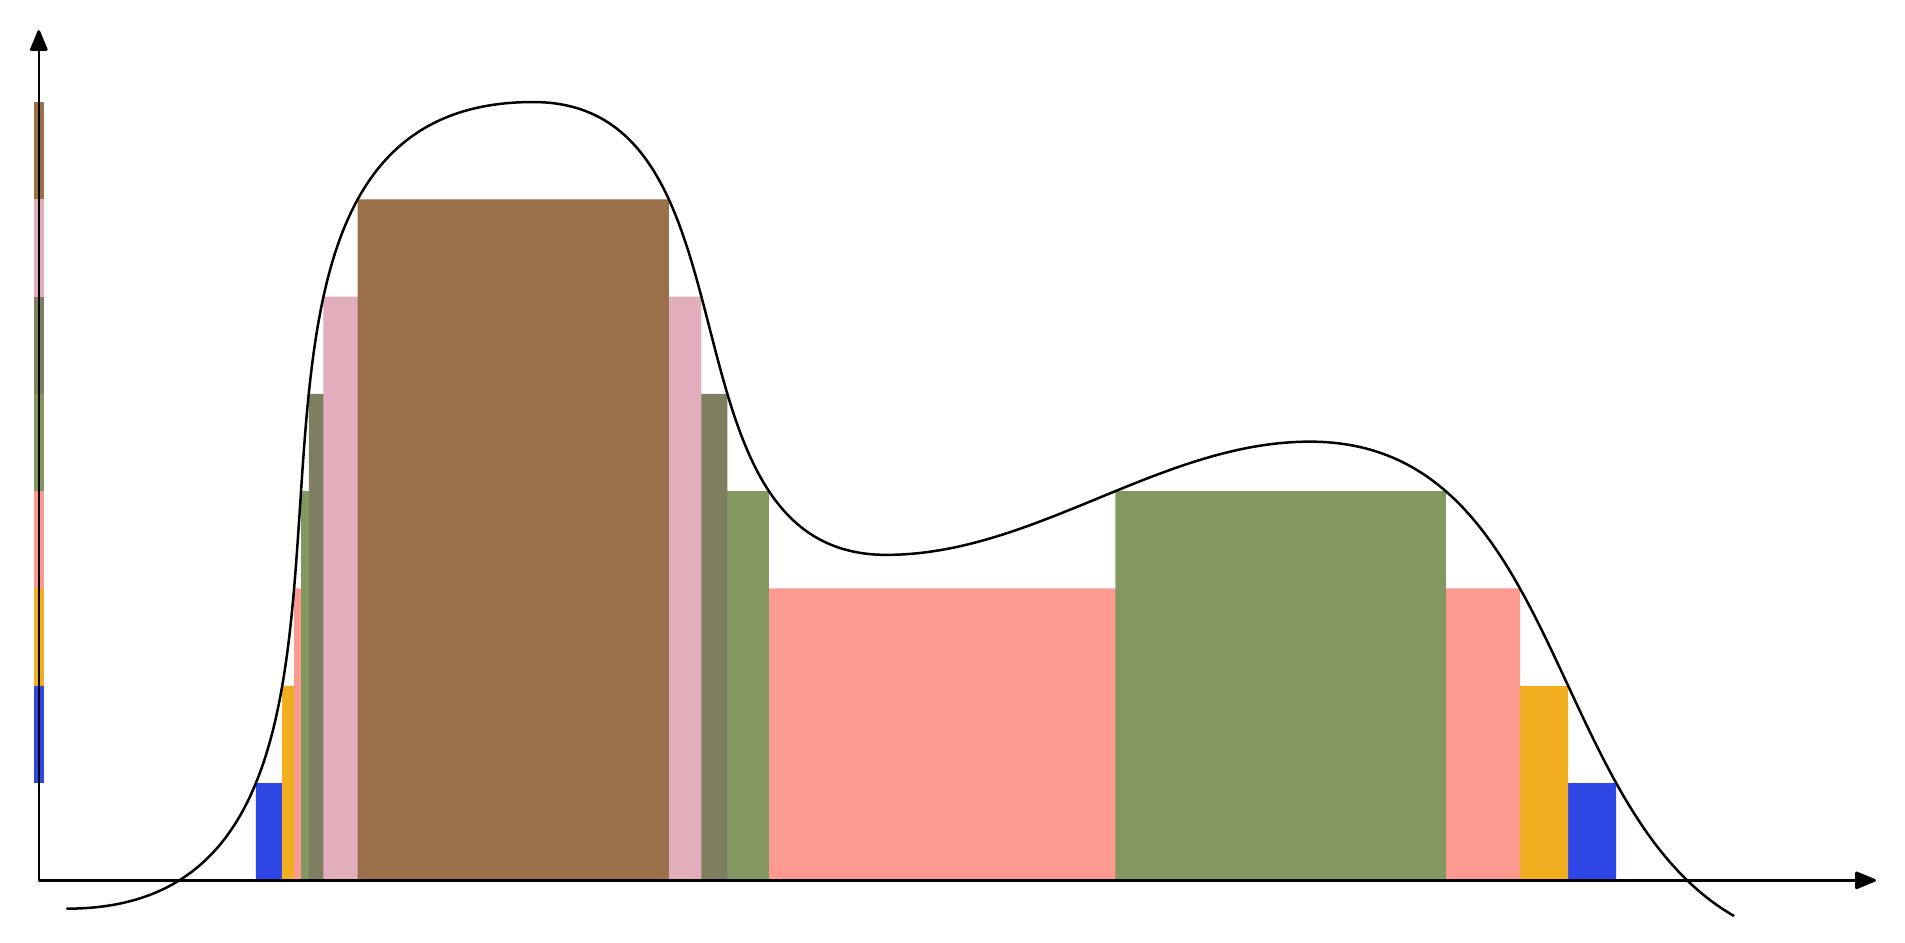
\includegraphics[width=1\linewidth]{fig1}
	\caption{$\varphi_7$.}
	\label{fig:simple-functions1}
\end{subfigure}
\\
	\begin{subfigure}{\linewidth}
	\centering
	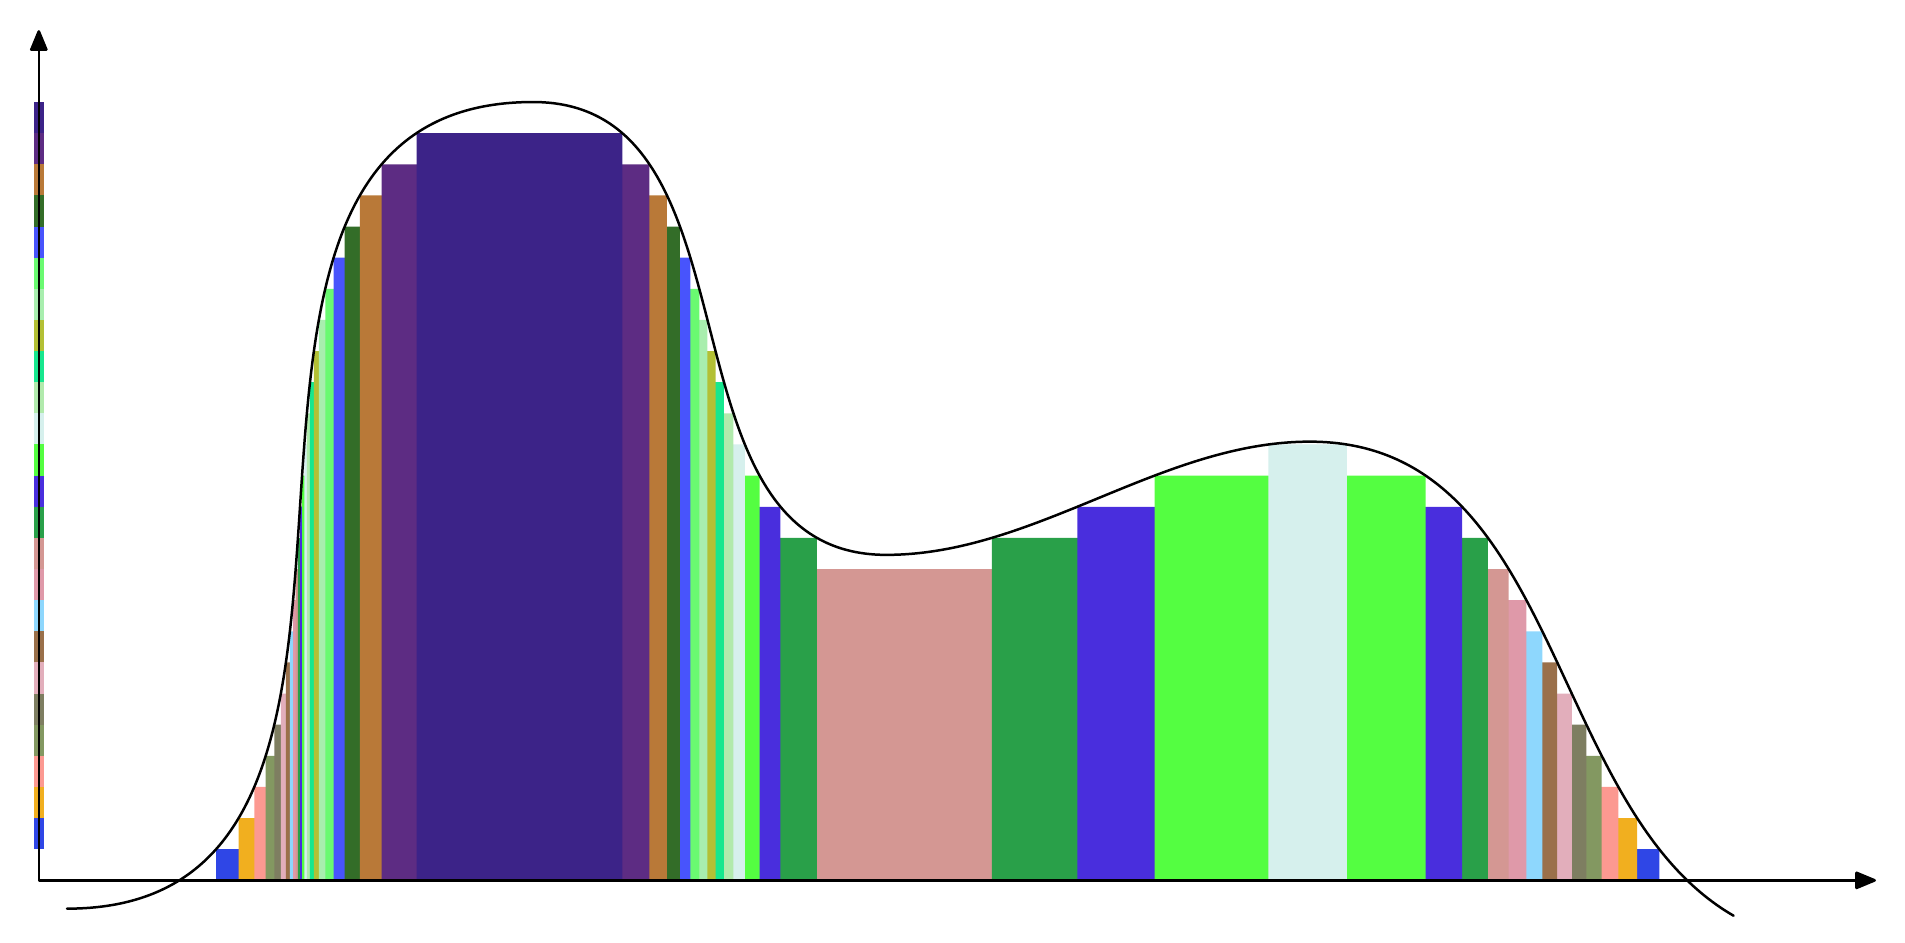
\includegraphics[width=1\linewidth]{fig2}
	\caption{$\varphi_{24}$.}
	\label{fig:simple-functions2}
\end{subfigure}
\end{center}
\caption{\href{https://tex.stackexchange.com/questions/667646/lebesgue-integral-on-tikz}{Approximation by simple functions.}}
\end{figure}
		\end{proof}
		\begin{prop}
			Let $(X,\mathcal{M},\mu)$ be a measure space and let $(X,\overline{\mathcal{M}},\overline{\mu})$ be its completion. If $f$ is a $\overline{\mathcal{M}}$-measurable function on $X$, there is an $\mathcal{M}$-measurable function $g$ such that $f=g\overline{\mu}$-almost everywhere.
		\end{prop}
		\end{itemize}
	\subsection{Riesz and Nagy's Functional Analysis}
		This section is a short digression to show the approach of \cite{riesz}.
		\begin{thm}[Lebesgue]
			Every monotonic function $f(x)$ posses a finite derivative at every point with the possible exception of the points $x$ of a set of measure zero, or, as it is often phrased, almost everywhere.
		\end{thm}
		A set of \textbf{\textit{measure zero}} is a set of values $x$ which can be covered by a finite number or by a denumerable sequence of intervals whose total length is arbitrarly small.
		
		Functions $f(x)$ continuous or not, for which the sum
		\[\sum_{ab}=\sum_1^n|f(x_k)-f(x_{k-1})|\]
		defined in terms of a decomposition of the interval $(a,b)$ into partial intervales $(x_{k-1},x_k)\;k=1,2,\ldots,n$, does not surpass a finit bound, independant of the particular choice of decomposition, are called \textbf{\textit{functions of bounded variation}}. The least upper bound is called the \textbf{\textit{total variation of $f(x)$ in the interval $(a,b)$}}.
		\begin{thm}[Lebesgue]
			Every function of bounded variation posses a finite derivative almost everywhere.
		\end{thm}
		\begin{thm}[Fubini]
			Let
			\[f_1(x)+f_2(x)+\ldots=s(x)\]
			be a convergent series all of whose terms are monotonic functions of the same type, defined on the interval $a\leq x\leq b$. Then
			\[f'_1(x)+f'_2(x)+\ldots=s'(x)\]
			except perhaps on a set of measure zero; that is, term by term differentiation is possible almost everywhere.
		\end{thm}
		\begin{thm}[Lebesgue]
			Almost all points of an arbitrary linear set are density points of that set.
		\end{thm}
		We include the following quote regarding Riemann integrals:
		\begin{quotation}[p. 23]
			\textit{(...) we arrive at a necessary condition that $f(x)$ be integrable in the Riemann sense, namely, that the function $f(x)$ be continuous almost everywhere.}
		\end{quotation}
		A \textbf{\textit{step function}} defined on an interval $(a,b)$ is a function having a constant value $c_k$ in each of a finite number of intervals $i_k$ of finite lenght $|i_k|$ and vanishing outside these intervals. We suppose the integral defined for these functions, as usual, by the sum $\sum c_k|i_k|$.
		\begin{lemma}\label{lemma:stepfunctionsA}
			For every sequence $\{\varphi_n(x)\}$ of step functions which decreases to 0 almost everywhere, the sequene of values of their integrals also tends to zero.
		\end{lemma}
		\begin{lemma}\label{lemma:stepfunctionsB}
			If for an increasing sequence of step functions $\{\varphi_n(x)\}$ the values of their integrals have a common bound, then the sequence $\{\varphi_n(x)\}$ tends almost everywhere to a finite limit.
		\end{lemma}
		Denote the class of stepfunctions by $C_0$ and the class of functions which are limits almost everywhere of the sequences $\{\varphi_n\}$ referred to in \cref{lemma:stepfunctionsB}. For $f(x)=\lim\varphi_n(x)$ define
		\[\int_a^bf(x)dx=\lim_{n\to \infty}\int_a^b\varphi_n(x)dx\]
		which does not depend on the particular choice of functions $\varphi_n$. In fact, if $\{\psi_n\}$ is increases almost everywhere to a limit function $g(x)\geq f(x)$, we also have
		\[\lim_{n\to\infty}\int_a^b\psi_n(x)dx\geq\lim_{n\to\infty}\int_a^b\varphi_n(x)dx\]
		so that if $g(x)=f(x)$ almost everywhere is implied.
	\subsection{Integration}
		In this section we continue reading \cite{folland}.
		
		Fix a measure space $(X,\mathcal{M},\mu)$ and define
		\[L^+=\text{ the space of all measurable functions from }X\text{ to }[0,\infty].\]
		If $\varphi$ is a simple function in $L^+$ with standard representation $\varphi=\sum_{j=1}^na_j\chi_{E_j}$, we definde the \textbf{\textit{integral of $\varphi$}} by
		\[\int\varphi d\mu=\sum_{j=1}^n a_j\mu(E_j)\]
		with the convention that $0\cdot\infty=0$. It may happen that $\int\varphi d\mu=\infty$.
		
		\begin{prop}Let $\varphi$ and $\psi$ be simple functions in $L^+$.
			\begin{enumerate}
				\item If $c\geq0$, then $\int c\varphi=c\int\varphi$.
				\item $\int(\varphi+\psi)=\int\varphi+\int\psi$.
				\item If $\varphi\leq\psi$ then $\int\varphi\leq\int\psi$.
				\item The map $A\mapsto\int_Ad\mu$ is a measure on $\mathcal{M}$.
			\end{enumerate}
		\end{prop}
		We now extend the integral to all functions in $L^+$ by defining
		\[\int fd\mu=\sup\left\{\int\varphi d\mu:0\leq\varphi\leq f,\varphi\text{ is simple}\right\}.\]
		\begin{remark}
			In \cite{riesz} the integral of $f$ is the \textit{limit} of the integrals of simple functions.
		\end{remark}
		\begin{remark}
			It is obvious from the definition that if $f\leq g$ then $\int f\leq\int g$ and $\int cf=c\int f$ for all $c\in[0,\infty)$.
		\end{remark}
		\begin{thm}[Monotone convergence, Beppo Levi, as in Folland]
			If $\{f_n\}$ is a sequence in $L^+$ (the set of measurable functions with values on $[0,\infty]$) such that $f_j\leq f_{j+1}$ for all $j$ and $f=\lim_{n\to\infty}f_n$, then $\int f_n\to\int f$.
		\end{thm}
		\begin{thm}[Monotone convergence, Beppo Levi, as in Brezis]
			Let $(f_n)$ be a seuence of functions in $L^1$ that satisfy
			\begin{enumerate}
				\item $f_1\leq f_2\leq\ldots\leq f_n\leq f_{n+1}\leq\ldots$ a.e. on $\Omega$,
				\item $\sup_n\int f_n<\infty$.
			\end{enumerate}
			Then $f_n(x)$ converges a.e. on $\Omega$ to a finite limit, which we denote by $f(x)$. The function $f$ belongs to $L^1$ and $\Vert f_n-f\Vert_1\to0$.
		\end{thm}
		\begin{proof}[Proof of the first statement]
			Since $\int f_n\leq\int f$ for all $n$, we have $\lim\int f_n\leq\int f$. To establish the reverse inequality fix $\alpha\in (0,1)$, let $\varphi$ be a simple function with $0\leq\varphi\leq f$ and $E_n=\{x:f_n(x)\geq\alpha\varphi(X)\}$. That is $E_n$ is the set of points in $X$ where the approximating function $f_n$ has a value greater than $\alpha\varphi(x)$.
			
			Then $\{E_n\}$ is an increasing sequence of measurable sets {\color{orange}...}
		\end{proof}
		\begin{thm}[Aditivity of the integral]
			If $\{f_n\}$ is a finit or infinite sequence in $L^+$ and $f=\sum_nf_n$ then $\int f=\sum_n\int f_n$.
		\end{thm}
		\begin{prop}
			If $f\in L^+$ then $\int f=0$ if and only if $f=0$ a.e.
		\end{prop}
		\begin{coro}
			If $\{f_n\}\subset L^+$ and $f_n(x)$ increases to $f(x)$ for a.e. $x$, then $\int f=\lim \int f$.
		\end{coro}
		\begin{lemma}[Fatou]
			If $\{f_n\}$ is any sequence in $L^+$, then
			\[\int\liminf f_n\leq\liminf\int f_n.\]
		\end{lemma}
		\begin{proof}
			For each $k\geq1$, we have $\inf_{n\geq k}f_n\leq f_j$ for $j\geq k$, so that $\int \inf_{n\geq k}f_n\leq\int f_j$ for $j\geq k$, and hence $\int \inf_{n\geq k}f_n\leq\inf_{j\geq k}\int f_j$. As $k\to\infty$,
			\[\int\liminf f_n=\int\lim_{k\to\infty}\inf_{n\geq k}f_n\overset{\text{m.c.t.}}{=}\lim_{k\to\infty}\int\inf_{n\geq k}f_n\leq\lim_{k\to\infty}\inf_{j\geq k}\int f_j=\liminf\int f_n\]
			by the monotone convergence theorem.
		\end{proof}
		\begin{coro}
			If $\{f_n\}\subset L^+$, $f\in L^+$ and $f_n\to f$ a.e., then $\int f\leq\liminf\int f_n$.
		\end{coro}
		\begin{prop}
			If $f\in L^+$ and $\int f<\infty$, then $\{x:f(x)=\infty\}$ is a null set and $\{x:f(x)>0\}$ is $\sigma$-finite.
		\end{prop}
		We may extender the former integral to real-valued functions as follows. If $f^+$ and $f^-$ are the positive and negative parts of $f$ and at least one of $\int f^+$ and $\int f^-$ is finite, we define
		\[\int f=\int f^+-\int f^-.\]
		If $\int f^+$ and $\int f^-$ are both finite we say $f$ is \textbf{\textit{integrable}}. Since $|f|=f^++f^-$, it is clear that $f$ is integrable if and only if $\int|f|<\infty$.
		\begin{prop}
			The set of integrable real-valued functions on $X$ is a real vector space and the integral is a linear functional on it.
		\end{prop}
		If $f$ is a complex-valued measurable function, we say that $f$ is \textbf{\textit{integrable}} if $\int|f|<\infty$. Since $|f|\leq|\operatorname{Re}f|+|\operatorname{Im}f|\leq2|f|$, $f$ is integrable if and only if $\operatorname{Re}f$ and $\operatorname{Im}f$ are both integrable, and we define
		\[\int=\int\operatorname{Re}f+i\int\operatorname{Im}f.\]
		The set of al complex-valued integrable functions is a complex vector space and the integral is a complex-linear functional on it. We denote this space by $L^1$, $L^1(\mu)$, $L^1(X,\mu)$ or $L^1(X)$.
		\begin{prop}
			If $f\in L^1$, then $|\int f|\leq \int|f|$.
		\end{prop}
		\begin{prop}\leavevmode
			\begin{enumerate}
				\item If $f\in L^1$, then $\{x:f(x)\neq0\}$ is $\sigma$-finite.
				\item If $f,g\in L^1$, then $\int_E f=\int_E g$ for all $E\in\mathcal{M}$ if and only if $\int|f-g|=0$ if and only if $f=g$ almost everywhere.
			\end{enumerate}
		\end{prop}
		This proposition shows that for the purposes of integration it makes no difference if we alter functions on null sets. With this in mind, we redefine $L^1$ \textbf{\textit{as the set of equivalence classes of a.e.-defined integrable functions on $X$}}, where $f$ and $g$ are considered equivalent if $f=g$ a.e.
		
		This new definition has two advantages. First, that if $\overline{\mu}$ is the completion of $\mu$, there is one-to-one correspondance between $L^1(\overline{\mu})$ and $L^1(\mu)$ by \cref{prop:?}, and we shall identify those spaces. Second, $L^1$ is a metric space with distance funcion $\rho(f,g)=\int|f-g|$: the triangle inequality is easily verified, and obviously $\rho(f,g)=\rho(g,f)$, but to prove that $\rho(f,g)=0$ only when $f=g$ we must identify functions that are equal a.e. We shall refer to convergence with respect to this metric as \textbf{\textit{convergence in $L^1$}}.
		\begin{thm}[Dominated Convergence, Lebesgue, as in Folland]
			Let $\{f_n\}$ be a sequence in $L^1$ such that $f_n\to f$ a.e. and there exists a nonnegative $g\in L^1$ such that $|f_n|\leq g$ a.e. for all $n$. Then $f\in L^1$ and $\int f_n\to \int f$.
		\end{thm}
		\begin{proof}
			By Fatou's Lemma.
		\end{proof}
		\begin{thm}[Dominated Convergence, Lebesgue, as in Brezis]
			Let $(f_n)$ be a sequence of functions in $L^1$ that satisfy
			\begin{enumerate}
				\item $f_n(x)\to f(x)$ a.e. on $\Omega$,
				\item there is a function $g\in L^1$ such that for all $n$, $|f_n(x)|\leq g(x)$ a.e. on $\Omega$.
			\end{enumerate}
			Then $f\in L^1$ and $\Vert f_n-f\Vert_1\to0$.
		\end{thm}
		\begin{remark}
			By comparing the statements of the Monotone Convergence and Dominated Convergence theorems in Folland and Brezis, we suspect that $\Vert f_n-f\Vert_1\to 0\iff \int f_n\to \int f$. At least one of the implications is straightforward:
			\begin{align*}
				\Vert f_n-f\Vert_1\to 0&\iff \int |f_n-f|\to0\\
				&{\color{orange}\implies}\left|\int (f_n-f)\right|\to0\\
				&\iff \left|\int f_n-\int f\right|\to0\\
				&\iff\int f_n\to\int f
		\end{align*}
		\end{remark}
		\begin{thm}
			Suppose that $\{f_j\}$ is a sequence in $L^1$ such that $\sum_{j=1}^\infty\int|f_j|<\infty$. Then $\sum_{j=1}^\infty f_j$ converges a.e. to a function in $L^1$, and $\int\sum_{j=1}^\infty f_j=\sum_{j=1}^\infty\int f_j$.
		\end{thm}
		\begin{proof}
			By the Dominated Convergence Theorem.
		\end{proof}
		\begin{thm}
			Integrable simple functions are dense in $L^1$. That is, for every $f\in L^1$ and $\varepsilon>0$ there is an integrable simple function $\varphi=\sum a_j\chi_{E_j}$ such that $\int|f-\varphi|d\mu<\varepsilon$.
			
			If $\mu$ is a Lebesgue-Stieltjes measure on $\R$, the sets $E_j$ in the definition of $\varphi$ can be taken to be finite unions of open intervales, and there is a continuous function $g$ \textbf{that vanishes outside a bounded interval} such that $\int|f-g|d\mu<\varepsilon$.
		\end{thm}
		\begin{proof}
			By the Dominated Convergence Theorem.
		\end{proof}
		
		
		The \textbf{\textit{Lebesgue integral}} is the integral we have developed then the measure is the Lebesgue measure.
		
	\subsection{Riemann and Lebesgue integrals}
		In this section we briefly compare the Riemann and Lebesgue integrals using Darboux's characterization of the riemann integral in terms of upper and lower sums, wich we now recall. Let $[a,b]$ be a compact interval. By a \textbf{\textit{partition of $[a,b]$}} we mean an inifinite sequence $P=\{t_j\}_{0}^{n}$. such that $a=t_0<t_1<\ldots<t_n=b$. Let $f$ be an arbitrary real-valued function on $[a,b]$. For each partition $P$ we define
		\[S_Pf=\sum_{j=0}^nM_j(t_j-t_{j-1}),\qquad s_Pf=\sum_{j=0}^nm_j(t_j-t_{j-1}),\]
		where $M_j$ and $m_j$ are the supremum and infimum of $f$ on $[t_{j-1},t_k]$. Then we define
		\[\overline{I}_a^b=\inf_PS_Pf,\qquad\underline{I}^b_a(f)=\sup_Ps_Pf.\]
		If $\overline{I}^b_a(f)=\underline{I}_a^b(f)$, their common value is the \textbf{\textit{Riemann integral $\int_a^bf$}} and $f$ is called \textbf{\textit{Riemann integrable}}.
		
		\begin{thm}
			Let $f$ be a bounded real-valued function on $[a,b]$.
			\begin{enumerate}
				\item If $f$ is Riemann integrable, then $f$ is Lebesgue measurable (and hence integrable on $[a,b]$ since it is bounded), and the integrals coincide.
				\item $f$ is Riemann integrable if and only if $\{x\in [a,b]:f\text{ is discontinuous at }x\}$ has Lebesgue measure zero.
			\end{enumerate}
		\end{thm}
		\begin{proof}
			Uses the Dominated Convergence Theorem.
		\end{proof}
				%RIEMANN VS LEBESGUE INTEGRAL FIGRURE
			\begin{figure}[H]
				\begin{subfigure}{0.5\linewidth}
					\begin{center}
						\[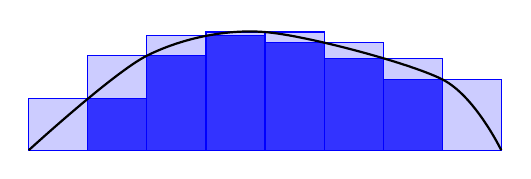
\begin{tikzpicture}
							\begin{scope}[scale=1.5]
								\draw[thick,name path=A] plot[smooth] coordinates {(0,0) (1,0.8) (2,1) (3.5,0.6) (4,0)};
								\begin{scope}[on background layer]
									\foreach \X [count=\Z] in {0,0.5,...,4}
									{\path[name path global=v-\Z,overlay] (\X,0) --  (\X,0|-current bounding box.north);
										\draw[name intersections={of=A and v-\Z,by=i-\Z},blue,fill=blue!20] 
										\ifnum\Z>1
										let \p1=(i-\the\numexpr\Z-1),\p2=(i-\Z) in
										(\X-0.5,0) rectangle (\X,{max(\y1,\y2)})
										\fi;
										\draw[name intersections={of=A and v-\Z,by=i-\Z},blue,fill=blue!80] 
										\ifnum\Z>1
										let \p1=(i-\the\numexpr\Z-1),\p2=(i-\Z) in
										(\X-0.5,0) rectangle (\X,{min(\y1,\y2)})
										\fi;}
								\end{scope}
							\end{scope}
						\end{tikzpicture}\]
						\caption{Riemann integral}
					\end{center}
				\end{subfigure}
				\begin{subfigure}{0.5\linewidth}
					\begin{center}
						\[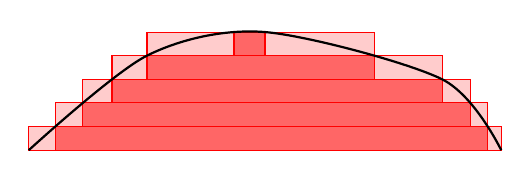
\begin{tikzpicture}
							\begin{scope}[yshift=-2cm,scale=1.5]
								\draw[thick,name path=B] plot[smooth] coordinates {(0,0) (1,0.8) (2,1) (3.5,0.6) (4,0)};
								\begin{scope}[on background layer]
									\foreach \Y [count=\Z] in {0,0.2,0.4,0.6,0.8,1}
									{\path[name path global=h-\Z,overlay] (0,\Y) --  (4,\Y);
										\draw[name intersections={of=B and h-\Z,by={i-\Z-1,i-\Z-2}},red,fill=red!20] 
										\ifnum\Z>1
										let \p1=(i-\the\numexpr\Z-1\relax-1),\p2=(i-\the\numexpr\Z-1\relax-2),
										\p3=(i-\Z-1),\p4=(i-\Z-2)
										in
										({min(\x1,\x3)},\Y-0.2) rectangle ({max(\x2,\x4)},\Y)
										\fi;
										\draw[name intersections={of=B and h-\Z,by={i-\Z-1,i-\Z-2}},red,fill=red!60] 
										\ifnum\Z>1
										let \p1=(i-\the\numexpr\Z-1\relax-1),\p2=(i-\the\numexpr\Z-1\relax-2),
										\p3=(i-\Z-1),\p4=(i-\Z-2)
										in
										({max(\x1,\x3)},\Y-0.2) rectangle ({min(\x2,\x4)},\Y)
										\fi;
									}
								\end{scope}
							\end{scope}
						\end{tikzpicture}\]
						\caption{Lebesgue integral}
					\end{center}
				\end{subfigure}
			\end{figure}
		
		\begin{remark}
			There are two main advantages of Lebesgue integration over Riemann integration. First, the convergence theorems, which do not hold for Riemann integrals. Second, that a wider class of functions may be integrated, which ultimately results in the completeness of certain function spaces.
		\end{remark}
		
		
	\subsection{Modes of convergence}
		Of course uniform convergence implies pointwise convergence, which in turn implies almost everywhere convergence, but these modes of convergence do not imply convergence in $L^1$ or vice versa.
		
		For example, $f_n=\frac{1}{n}\chi_{(0,n)}$ converges uniformly, pointwise and almost everywhere to $0$, but $\int|f_n|=1$ for all $n$. It is possible to find a function that converges in $L^1$ but does not converge pointwise.
		
		The dominated convergence theorem states that if $f_n\to f$ a.e. and $|f_n|\leq g\in L^1\;\forall n$, then $f\in L^1$. We also have that $f_n\to f$ in $L^1$, since $|f_n-f|\leq2g$. We shall see below that if $f_n\to f$ in $L^1$ then some subsequence converges to $f$ a.e.
		
		Now we introcues another mode of convergence. We say that a sequence $\{f_n\}$ of measurable complex-valued functions on $(X,\mathcal{M},\mu)$ is \textbf{\textit{Cauchy in measure}} if for every $\varepsilon>0$, 
		\[\mu(\{x:|f_n(x)-f_m(x)|\geq\varepsilon\})\to0\;\text{ as }m,n\to\infty,\]
		and that $\{f_n\}$ \textbf{\textit{converges in measure}} to $f$ if for every $\varepsilon>0$,
		\[\mu(\{x:|f_n(x)-f_m(x)|\geq\varepsilon\})\to0\;\text{as }n\to\infty.\]
		
		While our example sequence, $f_n=\frac{1}{n}\chi_{(0,n)}$ converges to zero in measure, the sequence $f_n=\chi_{[n,n+1]}$ is not Cauchy in measure.
		
		\begin{prop}
			If $f_n\to f$ in $L^1$, then $f_n\to f$ in measure.
		\end{prop}
		\begin{remark}
			The converse is false by the sequence $f_n=\frac{1}{n}\chi_{(0,n)}$.
		\end{remark}
		\begin{thm}
			Suppose that $\{f_n\}$ is Cauchy in measure. Then there is a measurable function $f$ such that $f_n\to f$ in measure, and there is a subsequence $\{f_{n_j}\}$ that converges to $f$ a.e. Moreover, if also $f_n\to g$ in measure, then $g=f$ a.e.
		\end{thm}
		\begin{remark}
			Bear in mind that a metric space is complete if all Cauchy sequences converge, and that we expect the space of real-valued functions to be complete since $\R$ is complete.
		\end{remark}
		\begin{remark}
			As an extra reminder, we recall that Cauchy sequences of real numbers are bounded, so that by the Bolsano-Weierstrass theorem they have convergent subsequences, which implies that they are convergent (since they are Cauchy).
		\end{remark}
		\begin{thm}
			If $f_n\to f$ in $L^1$, then there is a subsequence $f_{n_j}$ that converges to $f$ a.e.
		\end{thm}
		\begin{remark}
			This result may be thought as a kind of \textit{$L^1$-to-a.e. sequential compactness}.
		\end{remark}
		While, as we have said, a.e. convergence does not imply convergence in measure, the conclusion is true in a finite measure space. In fact, something stronger holds:
		\begin{thm}[Egoroff]
			Suppose that $\mu(X)<\infty$ and $f_1,f_2,\ldots$ and $f$ are measurable complex-valued functions on $X$ such that $f_n\to f$ a.e. Then $f_n$ converges to $f$ \textbf{\textit{almost uniformly}}, that is, for every $\varepsilon>0$ there exists $E\subset X$ such that $\mu(E)<\varepsilon$ and $f_n\to f$ on $E^c$. (Almost uniform convergence implies a.e. convergence and convergence in measure.)
		\end{thm}
	\subsection{Product measures}
	First we recall the construction of the product $\sigma$-algebra seen in \cref{subsec:sigma-algebras}. Let $\{X_\alpha\}_{\alpha\in A}$ is a collection of nonempty sets, $X=\prod_\alpha X_\alpha$ and $\pi_\alpha:X\to X_\alpha$ the coordinate functions. If $\mathcal{M}_\alpha$ is a $\sigma$-algebra on $X_\alpha$, the \textbf{\textit{product $\sigma$-algebra}} on $X$ is the $\sigma$-algebra generated by
	\[\{\pi_\alpha(E_\alpha):E_\alpha\in\mathcal{M}_\alpha,\alpha\in A\}\]
	We denote this $\sigma$-algebra by $\bigotimes_{\alpha\in A}\mathcal{M}_\alpha$.
	\begin{prop}
		$\bigotimes_{\alpha\in A}\mathcal{M}_\alpha$ is generated by $\{\prod_{\alpha\in A}E_\alpha:E_\alpha\in\mathcal{M}\}$. 
	\end{prop}
	
	In this section we consider two measure spaces $(X,\mathcal{M},\mu)$ and $(Y,\mathcal{N},\nu)$ and construct a measure on $\mathcal{M}\otimes\mathcal{N}$, the \textbf{\textit{product measure of $\mu$ and $\nu$}}.
	
	To begin with we define a \textbf{\textit{(measurable) rectangle}} to be a set of the form $A\times B$ where $A\in\mathcal{M}$ and $B\in\mathcal{N}$. As we have just recalled, the collection of finite disjoint unions of rectangles $\mathcal{A}$  is an algebra, and it generates $\mathcal{M}\otimes\mathcal{N}$.
	
	Constructing the produc measure is done by constructing first a premeasure. We consider a rectangle $A\times B$ that is finite or countable disjoint union of rectangles $A_j\times B_j$. Using aditivity of the integral we find that $\mu(A)\nu(B)=\sum\mu(A_j)\nu(B_j)$. Then we define for an element $E\in \mathcal{A}$ that is the disjoint union of rectangles $A_1\times B_1,\ldots,A_n\times B_n$, the function $\pi(E)=\sum_{j=1}^n\mu(A_j)\nu(E_j)$. Then $\pi$ is well defined on $\mathcal{A}$ and is a premeasure.
	
	By \cref{thm:premeasure}, there is an outer measure on $X\times Y$ whose restriction to $\mathcal{M}\times\mathcal{N}$ is a measure that extends $\pi$, which we call the \textbf{\textit{product measure $\mu\times\nu$ of $\mu$ and $\nu$}}. Moreover, if $\mu$ and $\nu$ are $\sigma$-finite (they can be seen as a countable union of sets of finite measure), so is $\mu\times\nu$. In this case, $\mu\times\nu$ is the unique measure on $\mathcal{M}\otimes\mathcal{N}$ such that $\mu\times\nu(A\times B)=\mu(A)\nu(B)$ for all rectangles $A\times B$.
	
	The same construction works for a finite number of factor spaces $(X_j,\mathcal{M}_j,\mu_j)$, yielding the produc measure $\mu_1\times\ldots\times\mu_n$ on $\mathcal{M}_1\otimes\ldots\otimes\mathcal{M}_n$. And again, if the $\mu_j$ are $\sigma$-finite, the product measure is uniquely determined.
	
	Let $(X,\mathcal{M},\mu)$ and $(Y,\mathcal{N},\nu)$ be two measure spaces. If $E\subset X\times Y$, define for $x\in E$ and $y\in Y$ the \textbf{\textit{$x$-section $E_x$}} and the \textbf{\textit{$y$-section $E^y$}} by
	\[E_x=\{y\in Y:(x,y)\in E\}\qquad E^y=\{x\in X:(x,y)\in E\}.\]
	Also, if $f$ is a function on $X\times Y$ we define the \textbf{\textit{$x$-section $f_x$}} and the \textbf{\textit{$y$-section $f^y$}} of $f$ by
	\[f_x(y)=f^y(x)=f(x,y).\]
	\begin{prop}\leavevmode
		\begin{enumerate}
			\item If $E\in \mathcal{M}\times\mathcal{N}$, then $E_x\in \mathcal{N}$ for all $x\in X$ and $E^y\in\mathcal{M}$ for all $y\in Y$.
			\item If $f$ is in $\mathcal{M}\otimes\mathcal{N}$-measurable, then $f_x$ is $\mathcal{N}$-measurable for all $x\in X$ and $f^y$ is $\mathcal{M}$-measurable for all $y\in Y$.
		\end{enumerate}
	\end{prop}
	\begin{thm}\label{thm:Fubini-Tonelli-previous}
		Suppose $(X,\mathcal{M},\mu)$ and $(Y,\mathcal{N},\nu)$ are $\sigma$-finite measure spaces. If $E\in\mathcal{M}\otimes\mathcal{N}$, then the functions $x\mapsto\nu(E_x)$ and $y\mapsto\mu(E^y)$ are measurable on $X$ and $Y$, respectively, and
		\[\mu\times\nu(E)=\int\nu(E_x)d\mu(x)=\int\mu(E^y)d\nu(y).\]
	\end{thm}
	\begin{proof}
		Uses the \textbf{\textit{Monotone Class Lemma}}, and the Monotone Convergence and Dominated Convergence theorems.
	\end{proof}
	\begin{thm}[Fubini-Tonelli, as in Folland] Suppose that $(X,\mathcal{M},\mu)$ and $(Y,\mathcal{N},\nu)$ are $\sigma$-finite measure spaes.
	\begin{enumerate}
		\item \textbf{(Tonelli.)} If $f\in L^+(X\times Y)=\text{ the set of measurable functions from }X\times Y\text{ to }[0,\infty]$, then the functions
			\[g(x)=\int f_xd\nu\quad\text{and}\quad h(y)=\int f^yd\mu\]
		are in $L^+(X)$ and $L^+(Y)$ respectively, and
		\begin{equation}\label{eq:Tonelli}
			\int fd(\mu\times\nu)=\int\left(\int f(x,y)d\nu(y)\right)d\mu(x)=\int\left(\int f(x,y)d\mu(x)\right)d\nu(y).
		\end{equation}
		\item \textbf{(Fubini.)} If $f\in L^1(\mu\times\nu)$, then $f_x\in L^1(\nu)$ for a.e. $x\in X$, $f^y\in L^1(\mu)$ for a.e. $y\in Y$, the a.e.-defined functions $g$ and $h$ are $L^1(\mu)$ and $L^1(\nu)$, respectively, and \cref{eq:Tonelli} holds.
	\end{enumerate}
	\end{thm}
	\begin{proof}
		By \cref{thm:Fubini-Tonelli-previous} and the Monotone Convergence Theorem.
	\end{proof}
	
	\begin{thm}[Tonelli, as in Brezis]
		Let $F(x,y):\Omega_1\times \Omega_2\to\R$ be a measurable function satisfying
	 	\[\int_{\Omega_1}|F(x,y)|d\mu_2<\infty\quad\text{for a.e. } x\in\Omega_1\]
		and
	 	\[\int_{\Omega_1}d\mu_1\int_{\Omega_2}|F(x,y)|d\mu_2<\infty.\]
		Then $F\in L^1(\Omega_1\times \Omega_2)$.
			
		{\color{persiangreen}Roughly speaking: if a slice of $F$ is integrable, then $F$ is integrable.}
	\end{thm}
	
	\begin{thm}[Fubini, as in Brezis]
		Assume that $F\in L^1(\Omega_1\times\Omega_2)$. Then for a.e. $x\in\Omega_1$, $F(x,y)\in L^1_y(\Omega_2)$ and $\int_{\Omega_2}F(x,y)d\mu_2\in L^1_x(\Omega_1)$. Similarly, for a.e. $y\in\Omega_2$, $F(x,y)\in L^1_x(\Omega_1)$ and $\int_{\Omega_1}F(x,y)d\mu_1\int\in L^1_y(\Omega_2)$.
		
		Moreover, one has
		\[\int_{\Omega_1}d\mu_1\int_{\Omega_2}F(x,y)d\mu_2=\int_{\Omega_2}d\mu_2\int_{\Omega_1}F(x,y)d\mu_1=\iint_{\Omega_1\times\Omega_2}F(x,y)d\mu_1d\mu_2.\]
	\end{thm}
	
	\begin{remark}
		These theorems show that the integral of a function over a cartesian product may be obtained by fixing one variable, integrating the resulting one-variable function, and then varying the first variable.
	\end{remark}
	\begin{remark}
		The difference between the theorems appears to concern wether or not we suppose that the function is non-negative.
	\end{remark}

		\begin{thm}[2.44]
			\[\int f(x)dx=|\det T|\int f\circ T(x)dx\]
		\end{thm}
		\begin{thm}[2.47, diffeomorphisms]
			content...
		\end{thm}

\clearpage

\section{Point set topology}
	\subsection{Metric spaces}
	 A \textbf{\textit{metric}} on a set $X$ is a function $\rho:X\times X\to [0,\infty)$ such that
	\begin{enumerate}
		\item $\rho(x,x)=0$ if and only if $x=0$.
		\item $\rho(x,y)=\rho(y,x)$ for all $x,y\in X$.
		\item $d(x,z)\leq d(x,y)+d(y,z)$ for all $x,y,z\in X$.
	\end{enumerate}
	Two metrics $\rho_1$ and $\rho_2$ on a set $X$ are \textbf{\textit{equivalent}} if $C\rho_1\leq\rho_2\leq C'\rho_2$ for some $C,C'>0$.
	
	\begin{thm}Let $(X,d)$ and $(Y,d')$ be metric spaces. If $f:X\to Y$, the following are equivalent conditions for $f$ to be \textbf{\textit{continuous}}:
		\begin{enumerate}
			\item $\forall x\in X\forall\varepsilon>0\exists\delta>0:f(B_\delta(x))\subseteq B_\varepsilon(f(x))$
			\item $\forall x\in X\forall x_n\to x:f(x_n)\to f(x)$.
			\item $\forall F\subseteq Y$ open, $f^{-1}(F)$ is open.
			\item $\forall F\subseteq Y$ closed, $f^{-1}(F)$ is closed.
		\end{enumerate}
	\end{thm}
	If $f:(X,\rho)\to(Y,\rho')$ is such that
	\[\forall\varepsilon>0\exists\delta>0\forall x\in X:f(B_\delta(x))\subseteq B_\varepsilon(f(x))\]
	we say $f$ is \textbf{\textit{uniformly continuous}}.
	\begin{exer*}
		If $(Y,\rho')$ is complete and $f:A\to Y$ is uniformly continuous on $A\subset X$ and $\overline{A}=X$, then $f$ has a unique continuous extension $g:X\to Y$ which is uniformly continuous on $X$. Show that this is not true in general if $Y$ is not complete.
	\end{exer*}
	If $f:(X,\rho)\to(Y,\rho')$ is a bijective function such that for any $x,y\in X$, $\rho(x,y)=\rho'(f(x),f(y))$ we say $f$ is an \textbf{\textit{isometry}} and the two spaces are \textbf{\textit{isometric}}. A function $f:(X,\rho)\to (X,\rho)$ is a \textbf{\textit{contraction}} if there exists a $0<a<1$ such that $\rho(f(x),f(y))\leq a\rho(x,y)$ for any $x,y\in X$. Every contraction is continuous, and if $X$ is complete then any contraction has a unique fixed point.
	
	A sequence $\{x_n\}$ in $X$ \textbf{\textit{converges}} to $x$ if $\lim_{n\to\infty}\rho(x_n,x)=0$. A sequence $\{x_n\}$ in $X$ is called \textbf{\textit{Cauchy}} if $\lim_{n,m\to\infty}\rho(x_n,x_m)=0$, that is
	
	\[\forall\varepsilon>0\exists N\in\N\forall n,m>N:\rho(x_n,x_m)<\varepsilon.\]
	
	A subset $E\subseteq X$ is \textbf{\textit{complete}} if every Cauchy sequence in $E$ converges to its limit in $E$. If $(X,\rho)$ and $(X^*,\rho^*)$ are metric spaces and
	\begin{enumerate}
		\item $(X,\rho)$ is isometric to a subspace $(X,\rho^*)$ of $(X^*,\rho^*)$,
		\item The closure of $X_0$ is all of $X^*$ ($X_0$ is \textbf{\textit{everywhere dense}} or simply \textbf{\textit{dense}}),
	\end{enumerate}
	we say $(X^*,\rho^*)$ is the \textbf{\textit{completion}} of $(X,\rho)$.
	\begin{thm}
		Every metric space $(X,\rho)$ has a completion $(X^*,\rho^*)$. If $(X^{**},\rho^{**})$ is also a completion of $(X,\rho^*)$, then $(X^*,\rho^*)$ is isometric to $(X^{**},\rho^{**})$; that is, the completion of a space is unique up to isometry.
	\end{thm}
	\begin{proof}
		Consider equivalence classes of Cauchy sequences.
	\end{proof}
	
	\begin{prop}
		A closed subset of a metric space is complete, and a complete subset of an arbitrary metric space is closed.
	\end{prop}
	
	\subsection{Topological spaces}
	Let $X$ be a nonempty set. A \textbf{\textit{topology}} on $X$ is a family $\mathcal{T}$ of subsets of $X$ that contains $\varnothing$ and $X$ and is closed under arbitrary unions and finite intersections. (That is, if $\{U_\alpha\}_{\alpha\in X}\subset\mathcal{T}$ then $\bigcup_{\alpha\in A}U_\alpha\in\mathcal{T}$ and if $U_1,\ldots, U_n\in\mathcal{T}$ then $\bigcap_{j=1}^nU_j\in\mathcal{T}$.) The pair $(X,\mathcal{T})$ is called a \textbf{\textit{topological space}}.
	
	The memebers of $\mathcal{T}$ are called \textbf{\textit{open sets}} and their complements are called \textbf{\textit{closed sets}}. If $A\subseteq X$, the union of all open sets contained in $A$ is called the \textbf{\textit{interior}} of $A$, denoted by $A^o$; so that a point $x\in A^o$ when there is an open set $O$ contained in $A$ such that $x\in O$. The intersection of all closed sets containing $A$ is called the \textbf{\textit{closure}} of $A$. The difference $\bar{A}\backslash A^o=\bar{A}\cap\overline{A^c}$ is called the \textbf{\textit{boundary}} of $A$ and is denoted by $\partial A$.
	
	
	
	Following \cite{narici}, a point $x\in X$ is an \textbf{\textit{adherence point}} of the subset $E$ if every open set containing $x$ conatins a point of $E$. The set of all adherence points of $E$ is called the \textbf{\textit{closure}} of $E$ and it is denoted by $\overline{E}$. It is immediate that $E\subset\overline{E}$.
	\begin{prop}
		Let $X$ be a topological space and $A$ and $B$ subsets of $X$. Then
		\begin{enumerate}
			\item $A\subset B\implies\bar{A}\subset\bar{B}$.
			\item $\overline{A\cup B}\implies\bar{A}\cup\bar{B}$,
			\item $\bar{A}=\bar{\bar{A}}$.
			\item A subset $F$ of $X$ is closed if and only if $F=\overline{F}$.
		\end{enumerate}
	\end{prop}
	If $X$ is a topological space and $A$ is a subset of $X$, a point $x\in X$ is called a \textbf{\textit{limit point}} of $A$ if every open set containing $x$ contains a point of $A$ distinct from $x$. The set of all limit points of $A$ is denoted by $A'$ and is called the \textbf{\textit{derived set of $A$}}. Clearly, $\bar{A}=A\cup A'$, and, in view of the last item in the last proposition, $A$ is closed if and only if $A'\subset A$.
	
	A sequence of points $\{x_n\}$ in a topological space $X$ \textbf{\textit{converges}} to the point $x\in X$ if for every open set $O$ containing $x$ there exists an index $N$ (dependending on $O$) such that $x_n\in O$ for all $n>N$. That is, every open set containing $x$ must contain almost all (but a finite number) of the $x_n$.
	
	\begin{prop} Let $X_1$, $X_2$ and $X_3$ be topologial spaces. Let $f:X_1\to X_2$ and $g:X_2\to X_3$ be mappings.
		\begin{enumerate} 
			\item If $f$ and $g$ are continuous, then the composite mapping $gf$ is continuous.
			\item $f$ is continuous if and only if for every subset $A$ of $X$, $f\bar{A}\subset\overline{f(A)}$.
			\item Suppose $f$ is a 1:1, onto mapping. Then $f$ is a homeomorphism of $X_1$ onto $X_2$ is and only if, for all subsets $A$ of $X_1$, $f(\bar{A})=\overline{f(A)}$.
		\end{enumerate}
	\end{prop}
	
	
	If $\mathcal{T}_1$ and $\mathcal{T}_2$ are two topologies on a set $X$, we say $\mathcal{T}_1$ is \textbf{\textit{weaker}} (or \textbf{\textit{coarser}}) and $\mathcal{T}_2$ \textbf{\textit{stronger}} (or \textbf{\textit{finer}}) if $\mathcal{T}_1\subseteq\mathcal{T}_2$. $E\subseteq X$ is called \textbf{\textit{dense}} if $\overline{E}=X$ and \textbf{\textit{nowhere dense}} if $\overline{E}$ has empty interior. $X$ is called \textbf{\textit{separable}} if it has a countable dense subset. 
	
	\begin{enumerate}
		\item[$\operatorname{T}_0$] If $x\neq y$, there is an open set containing $x$ but not $y$, or an open set containing $y$ but not $x$.
		\item[$\operatorname{T}_1$] If $x\neq y$, there is an open set containint $y$ but not $x$. Equivalently, $\{x\}$ is closed for every $x\in X$.
		\item[$\operatorname{T}_2$] \textbf{(Hausdorff.)} If $x\neq y$ there are disjoint open sets $U$ and $V$ such that $x\in U$ and $y\in V$.
		\item[$\operatorname{T}_3$] \textbf{(Regular.)} $X$ is $\operatorname{T}_1$ and for any closed set $A\subset X$ and any $x\in A^c$ there are disjoint open sets $U,V$ with $x\in U$ and $a\subseteq V$.
		\item[$\operatorname{T}_{3\frac{1}{2}}$] \textbf{(Tychonoff, Completely regular.)} $X$ is $\operatorname{T}_1$ and for each closed $A\subseteq X$ and each $x\notin A$ there exists $f\in C(X,[0,1])$ such that $f(x)=1$ and $f=0$ on $A$.
		\item[$\operatorname{T}_4$] \textbf{(Normal.)} $X$ is $T_1$ and for any disjoint closed sets $A,B$ in $X$ there are disjoint open sets $U,V$ with $A\subseteq U$ and $B\subseteq V$.
	\end{enumerate}
	
	If $X$ is any set and $\{f_\alpha:X\to Y_\alpha\}_{\alpha\in A}$ is a family of maps from $X$ into some topological spaces $Y_\alpha$, there is a unique weakest topology $\tau$ on $X$ that makes all the $f_\alpha$ continuous called the \textbf{\textit{weak topology generated by $\{f_\alpha\}_{\alpha\in A}$}}. An example of this topology is the \textbf{\textit{product topology}} on $X=\prod_{\alpha\in A}X_\alpha$ with the projections.
	
	\begin{prop}\leavevmode
		\begin{itemize}
			\item If $X_\alpha$ is Hausdorff for each $\alpha\in A$ then $X=\prod_{\alpha\in A}$ is Hausdorff.
			\item If $X_\alpha$ and $Y$ are topological spaces, a function $f:Y\to X=\prod_{\alpha\in A}X_\alpha$ is continuous if and only iff $\pi_\alpha\circ f$ is continuous for each $\alpha$.
			\item If $X$ is a topological space, $A$ is a nonempty set and $\{f_n\}$ is a sequence in $X^A$, then $f_n\to f$ in the product topology if and only if $f_n\to f$ pointwise.
		\end{itemize}
	\end{prop}
	
	If $X$ is any set and $K=\R$ or $\C$, denote by $B(X,K)$ the \textbf{\textit{set of bounded $K$-valued functions on $X$}}, $C(X,K)$ the set of \textbf{\textit{continuous $K$-valued functions on $X$}}, and $BC(X,K)$ the \textbf{\textit{set of bounded continuous functions on $X$}}. If no field is specified we take it to be $\C$.
	
	For $f\in B(X)$ define the \textbf{\textit{uniform norm}} of $f$ to be
	\[\Vert f\Vert_u=\sup\{|f(x)|:x\in X\}\]
	Then the function $\rho(f,g)=|Vert f-g|Vert_u$ is a metric on $B(X)$. Convergence in this metric is simply uniform convergence:
	\[\{f_n\}\overset{u}{to}f\iff\forall\varepsilon>0\exists N\in\N\forall n>N\forall x\in X:|f_n(x)-f(x)|<\varepsilon\]
	$B(X)$ is complete with this metric since $\C$ is complete.
	
	\begin{prop}
		If $X$ is a topological space, $BC(X)$ is a closed subspace of $B(X)$ in the uniform metric; in particular $BC(X)$ is complete.
	\end{prop}
	\begin{lemma}[Urysohn]
		Let $X$ be a normal space. If $A$ and $B$ are disjoint closed sets in $X$, there exists $f\in C(X,[0,1])$ such that $f=0$ on $A$ and $f=1$ on $B$.
	\end{lemma}
	\begin{thm}[Tietze Extension Theorem]
		Let $X$ be a normal space. If $A$ is a closed subset of $X$ and $f\in C(A,[a,b])$, there exists $F\in C(X,[a,b])$ such that $F|A=f$.
	\end{thm}
	\begin{coro}
		If $X$ is normal, $A\subseteq X$ is closed and $f\in C(A)$, there exists $F\in C(X)$ such that $F|A=f$.
	\end{coro}
	Urysohn's lemma shows that every $\operatorname{T}_4$ space is completely regular ($\operatorname{T}_{3\frac{1}{2}}$).
	\begin{thm}[Dugundji]
		Sea $X$ un espacio metrizable, $A=\bar{A}\subset X$ y $L$ un espacio vectorial localmente convexo, y $V\subset L$ convexo. Entonces cualquier función $f:A\to V$ admite una extensión $F$.
		\[\begin{tikzcd}
			A\arrow[r,"f"]\arrow[hook,d]&V\\
			X\arrow[ur,dashed,"F",swap]
		\end{tikzcd}\]
		Además $\img F\subset\operatorname{conv}\img F$.
	\end{thm}
	
	\subsection{Compact spaces}
	
		A topological space $X$ is called \textbf{\textit{compact}} if whenever $\{U_\alpha\}_{\alpha\in A}$ is an open cover of $X$ there is a finite subset $B$ of $A$ such that $X=\bigcup_{\alpha\in B}U_\alpha$. A subset $Y\subseteq X$ is called \textbf{\textit{compact}} if it is compact in the relative topology and \textbf{\textit{precompact}} if its closure is compact.
		
		A family $\{F_\alpha\}_{\alpha\in A}$ of subsets of $X$ has the \textbf{\textit{finite intersection property}} if $\bigcap_{\alpha\in B}F_\alpha\neq\varnothing$ for all finite $B\subseteq A$.
		
		\begin{prop}\leavevmode
			\begin{itemize}
				\item A topological space $X$ is compact if and only if for every family $\{F_\alpha\}_{\alpha\in A}$ of closed sets with the finite intersection property, $\bigcap_{\alpha\in A}F_\alpha\neq\varnothing$.
				\item A closed subset of a compact space is compact.
				\item If $K$ is a compact subset of a Hausdorff space $X$ and $x\notin K$ then there are disjoint open sets $U,V$ such that $x\in U$ and $K\subseteq V$.
				\item Every compact subset of a Hausdorff space is closed.
				\item Every compact Hausdorff space is normal.
				\item If $X$ is compact and $f:X\to Y$ is continuous then $f(X)$ is compact.
				\item If $X$ is compact, then $C(X)=BC(X)$.
				\item If $X$ is compact and $Y$ is Hausdorff, then any continuous bijection $f:X\to Y$ is an homeomorphism.
			\end{itemize}
		\end{prop}
		A topological space $X$ is \textbf{\textit{countably compact}} if every countable open cover of $X$ has a finite subcover, and \textbf{\textit{sequentially compact}} if every sequence in $X$ has a convergent subsequence. For metric spaces compactness and sequential compactness are the equivalent. There exists no general relation between compactness and sequential compactness.
		
		\begin{thm}[Heine-Borel]
			A subset of $\R^n$ is compact if and only it is closed and bounded.
		\end{thm}
		\begin{thm}[Bolzano-Weierstrass]
			Every bounded sequence in $\R^n$ has a convergent subsequence. Equivalently, a subset of $\R^n$ is sequentially compact if and only if it is closed and bounded.
		\end{thm}
			\begin{thm}
			If $E$ is a subset of a metric space $(X,\rho)$, the following are equivalent:
			\begin{enumerate}
				\item $E$ is complete and \textbf{\textit{totally bounded}} (it can be covered by finitely many balls of radius $\varepsilon$).
				\item Every sequence in $E$ has a subsequence that converges to a point in $E$.
				\item If $\{V_\alpha\}_{\alpha\in A}$ is an open cover of $E$, then there is a finite subset $F\subseteq A$ such that $\{V_\alpha\}_{\alpha\in F}$ covers $E$.
			\end{enumerate}
		\end{thm}
		\begin{thm}
			If $(X,\rho)$ is a metric space and $A$ is compact, then $A$ is closed and bounded.
		\end{thm}
		We conclude with the approach of Narici.
		
		If $(X,\rho)$ is a metric space, $A\subseteq X$ is \textbf{\textit{relatively compact}} if $\overline{A}$ is compact. If $\varepsilon>0$, a subset $N\subset X$ is an \textbf{\textit{$\varepsilon$-net with respect to $A$}} if $\forall x\in A\exists n\in N:\rho(x,n)<\varepsilon$. $A$ is \textbf{\textit{totally boundad}} if for any $\varepsilon>0$ there exists a finite $\varepsilon$-net with respect to $A$.
		
		\begin{thm}
			Let $(X,\rho)$ be a metric space and $A\subseteq X$. If for every sequence of points from $A$ one can select a convergent subsequence, then $A$ is totally bounded.
		\end{thm}
		A set $A$ is \textbf{\textit{countably compact}} if every infinite subset of $A$ has a limit point in $A$. All compact sets are countably compact. $A$ is \textbf{\textit{sequentially compact}} if every sequence in $A$ has a subsequence that converges to a point in $A$. In a metric space, compactness is equivalent to countable and sequential compactness.
		
		\begin{thm} \label{thm:compactness-properties} Let $(X,\rho)$ be a metric space and $A\subseteq X$.
			\begin{enumerate}
				\item $A$ is relatively compact if and only if a convergent subsequence can be selected from every sequence of points in $A$. (We do not claim that the limit point is a member of $A$.)
				\item If $A$ is relatively compact, it is also totally bounded.
				\item If $(X,\rho)$ is complete and $A$ is totally bounded, then $A$ is relatively compact.
				\item If $A$ is compact then $A$ is closed and totally bounded.
			\end{enumerate}
		\end{thm}
		
	\subsection{Locally Compact Hausdorff spaces}
		
		A topological space is called \textbf{\textit{locally compact}} if every point has a compact neighbourhood (a set $A\subset X$ such that $x\in A^o$). We call locally compact Hausdorff spaces \textbf{\textit{LCH}} for short.
		\begin{prop}Let $X$ be a LCH space.
			\begin{itemize}
				\item If $U\subseteq X$ is open and $x\in U$, there is a compact neighbourhood $K$ of $x$ such that $K\subset U$.
				\item If $K\subseteq U\subseteq X$, with $K$ compact and $U$ open, there exists a precompact open $V$ such that $K\subseteq V\subset \overline{V}\subset U$.
				\item \textbf{(Urysohn's Lemma, Locally Compact Version.)} If $K\subset U\subseteq X$, there exists $f\in C(X,[0,1])$ such that $f=1$ on $K$ and $f=0$ outside a compact subset of $U$.
				\item Every LCH space is completely regular.
				\item \textbf{(Tietze Extension Theorem, Locally Compact Version)} If $K\subseteq X$ is compact and $f\in C(K)$, there exists $F\in C(X)$ such that $F|K=f$. $F$ may be taken to vanish outside a compact set.	
			\end{itemize}
		\end{prop}
		 If $f\in C(X)$, the \textbf{\textit{support of $f$}} is the closure of $\{x\in X:f(x)\neq0\}$ and denote $C_c(X):=\{f\in C(X):\operatorname{supp}f\text{ is compact}\}$. We say $f$ \textbf{\textit{vanishes at infinity}} if for every $\varepsilon>0$ the set $\{x:|f(x)|\geq\varepsilon\}$ is compact and define $C_0(X):=\{f\in C(X):f\text{ vanishes at infinity}\}$.
		 \begin{prop}
		 	If $X$ is an LCH space, $C_0(X)$ is the closure of $C_c(X)$ in the uniform metric.
		 \end{prop}
		 If $X$ is a topological space, there are many ways of topologizing $\C^X$. One way is the product topology, that is, the topology of pointwise convergence. Another is the \textbf{\textit{topology of uniform convergence}}, which is generated by the sets
		 \[\left\{g\in\C^X:\sup_{x\in X}|g(x)-f(x)|<n^{-1}\right\}\qquad n\in\N,f\in\C^X.\]
		 In view of a previous proposition (cite?), we know $C(X)$ is a closed subset of $\C^X$ with the topology of uniform convergence. Another topology is the \textbf{\textit{topology of uniform convergence on compact sets}}, generated by the sets
			 \[\left\{g\in\C^X:\sup_{x\in K}|g(x)-f(x)|<n^{-1}\right\}\qquad n\in\N,f\in\C^X,K\subseteq X\text{ compact}.\]
		\begin{prop}Let $X$ be an LCH space.
			\begin{itemize}
				\item If $E\subseteq X$, then $E$ is closed if and only if $E\cap K$ is closed for every compact $K\subseteq X$.
				\item $C(X)$ is a closed subspace of $\C^X$ in the topology of uniform convergence on compact sets.
				\item If $\{U_j\}_{j=1}^n$ is an open cover of a compact subset $K$ of $X$, then there is a partition of unity on $K$ subordinate to $\{U_j\}_{j=1}^n$ soncisting of compactly supported functions.
			\end{itemize}
		\end{prop}
		
		\begin{thm}[Urysohn Metrization Theorem]
			Every second countable normal space is metrizable.
		\end{thm}
		
	\subsection{Three compactness theorems}
		Recall that if $X=\prod_{\alpha\in A}X_\alpha$, an element $x\in X$ is just a mapping from $A$ to $\bigcup_{\alpha\in A}X_\alpha$, with $x(\alpha)$ the $\alpha$th coordinate of $x$.
		
		\begin{thm}
			If $\{X_\alpha\}_{\alpha\in A}$ is a family of compact topological spaces, then $X=\prod_{\alpha\in A}X_\alpha$ is compact with the produc topology.
		\end{thm}
		Let $X$ be a topological space and $\mathcal{F}\subseteq C(X)$ a family of complex-valued continuous functions on $X$. We say $\mathcal{F}$ is \textbf{\textit{equicontinuous at $x\in X$}} if for every $\varepsilon>0$ there is a neighbourhood $U$ of $x$ such that $|f(x)-f(y)|<\varepsilon$ for all $y\in U$ and all $f\in\mathcal{F}$; and \textbf{\textit{equicontinuous}} if it is equicontinuous at every $x\in X$. Also, $\mathcal{F}$ is \textbf{\textit{pointwise bounded}} if $\{|f(x)|:f\in\mathcal{F}\}$ is bounded for all $x\in X$.
	
		\begin{thm}[Arzelá-Ascoli I]
			Let $X$ be a compact Housdorff space. If $\mathcal{F}$ is an equicontinuous, pointwise bounded subset of $C(X)$, then $\mathcal{F}$ is totally bounded in the uniform metric, and the closure of $\mathcal{F}$ in $C(X)$ is compact.
		\end{thm}
		\begin{thm}[Arzelá-Ascoli II]
			Let $X$ be a locally compact Housdorff space. If $\{f_n\}$ is an equicontinuous, pointwise bounded sequence in $C(X)$, then there exists $f\in C(X)$ and a subsequence of $\{f_n\}$ that converges to $f$ uniformly on compact sets.
		\end{thm}
	\subsection{The Stone-Weierstrass Theorem}
		Recall that the Weierstrass theorem states that any continuous function on a compact interval $[a,b]$ is the uniform limit of polynomials on $[a,b]$. Throughout this subsection, $X$ will denote a compact Hausdorff space, and $C(X)$ is equipped with the uniform metric.
		
		A subset $\mathcal{A}$ of $C(X,\R)$ of $C(X)$ is said to \textbf{\textit{separate points}} if for every $x,y\in X$ with $x\neq y$ there exists $f\in \mathcal{A}$ such that $f(x)\neq f(y)$. $\mathcal{A}$ is called an \textbf{\textit{algebra}} if it is a real (resp. complex) vector subspace of $C(X,\R)$ (resp. $C(X)$) such that $fg\in \mathcal{A}$ whenever $f,g\in\mathcal{A}$. $\mathcal{A}$ is called a \textbf{\textit{lattice}} if $\max (f,g)$ and $\min (f,g)$ are in $\mathcal{A}$ whenever $f,g\in \mathcal{A}$. If $\mathcal{A}$ is an algebra or a lattice, so is its closure in the uniform metric.
		
		\begin{thm}[Stone-Weierstrass Theorem]
			Let $X$ be a compact Hausdorff space. If $\mathcal{A}$ is a closed subalgebra of $C(X,\R)$ that separates points, then either $A=C(X,\R)$ of $\mathcal{A}=\{f\in C(X,\R):f(x_0)=0\}$ for some $x_0\in X$. The first alternative holds if and only if $\mathcal{A}$ contains the constant functions.
		\end{thm}
		\begin{coro}
			Supoose $\mathcal{B}$ is a subalgebra of $C(X,\R)$ that separates points. If there exists $x_0\in X$ such that $f(x_0)=0$ for all $f\in\mathcal{B}$, then $\mathcal{B}$ is dense in $\{f\in C(X,\R):f(x_0)=0\}$. Otherwise, $\mathcal{B}$ is dense in $C(X,\R)$.
		\end{coro}
		The classical Weierstrass approximation theorem is the special case of this corollary where $X$ is the compact subset of $\R^n$ and $\mathcal{B}$ is the algebra of polynomials on $\R^n$ (restricted to $X$); here $\mathcal{B}$ contains the constant functions, so it is dense in $C(X,\R)$.
		
		The Stone-Weirstrass theorem, as stated, is false for complex-valued functions. We may show that $f(z)=\bar{z}$ cannot be approximately uniformly by polynomials on the unit circle.
		
		\begin{thm}[Complex Stone-Weirstrass Theorem]
			Let $X$ be a compact Hausdorff space. If $\mathcal{A}$ is a closed complex subalgebra of $C(X)$ that separates points and is closed under complex conjugation, then either $A=C(X)$ of $\mathcal{A}=\{f\in C(X):f(x_0)=0\}$ for some $x_0\in X$.
		\end{thm}
		Finally, there is a version of the Stone-Weirstrass theorem for noncompact LCH spaces. We state for real functions; the complex analogue is an immediate consequence.
		\begin{thm}[LCH Stone-Weirstrass Theorem]
			Let $X$ be a noncompact LCH space. If $\mathcal{A}$ is a closed complex subalgebra of $C_0(X,\R)$ that separates points, then either $A=C_0(X,\R)$ of $\mathcal{A}=\{f\in C_0(X,\R):f(x_0)=0\}$ for some $x_0\in X$.
		\end{thm}

\clearpage
\section{Inner product spaces}
	\subsection{Inner products}
	Let $X$ be a real or complex vector space.
	An \textbf{\textit{inner product}} on $X$ is a mapping
	\begin{align*}
		\langle-,-\rangle:X\times X\to F
	\end{align*}
	with the following properties:
	\begin{enumerate}
		\item[($\operatorname{I}_1$)] if $x,y\in X$ then $\langle x,y\rangle=\overline{\langle x,y\rangle}$;
		\item[($\operatorname{I}_2$)] if $\alpha,\beta$ are scalars, $\langle\alpha x+\beta y,z\rangle =\alpha\langle x,z\rangle+\beta\langle y,z\rangle$;
		\item[($\operatorname{I}_3$)] $\langle x,x\rangle\geq0$ for all $x\in X$ and equal to zero if and only if $x$ is the zero vector. (Since, by $\operatorname{I}_1$, $\langle x,x\rangle$ must be real.)
	\end{enumerate}
	\begin{examples}\leavevmode
		\begin{enumerate}
			\item Let $X=C[a,b]$ be complex-valued continuous functions on the closed interval $[a,b]$ with pointwise addition and scalar product. As the inner product of any two vectors $f$ and $g$ in this space take
		\[\langle f,g\rangle=\int_a^bf(x)\overline{g(x)}dx\]
		\item Let $X=l_2$, the set of all sequences of complex numbers $(a_1,a_2,\ldots)$ with the property that $\sum_{i=1}^\infty|a_i|^2<\infty$. As the inner product of any two vectors $x=(a_i)$ and $y=(b_i)$ in this space take
		\[\langle f,g\rangle=\sum_{i=1}^\infty a_i\overline{b}_i\]
		which converges by the Hölder inequality.
		
		\item Let $Y$ be the closed interval $[a,b]$, $S$ the Lebesgue measurable sets and $\mu$ the Lebesgue measure. Then, for the equivalence clasess of square-integrable functions (complex-valued) on $[a,b]$ we can take as the inner product of two clases $f$ and $g$,
				\[\langle f,g\rangle=\int_a^bf(x)\overline{g(x)}dx\]
		where the integral is the Lebesgue integral. This space is denoted by $L_2(a,b)$.
		\end{enumerate}
		\end{examples}
		\begin{thm}[Cauchy-Schwarz inequality]
			Let $X$ be an inner product space and let $x,y\in X$. Then
			\[|\langle x,y\rangle\leq\Vert x\Vert\Vert y\Vert\]
			with equality holding if and only if $x$ and $y$ are linearly independent.
		\end{thm}
	\subsection{Orthogonal projections}
	Two vectors $x,y\in X$ are \textbf{\textit{orthogonal}} if $\langle x,y\rangle=0$.
		\begin{examples}\leavevmode
	\begin{enumerate}
		\item In $L_2(–\pi,\pi)$, the collection (or any subset thereof)
			\[x_n=\frac{1}{\sqrt{2\pi}}e^{int},\qquad n=0,\pm1,\ldots\]
			is an orthonormal set of vectors.
			\begin{proof}
				For any $n\in\Z$,
				\[\int_{-\pi}^\pi x_n\overline{x}_ndt=\frac{1}{2\pi}\int_{-\pi}^\pi e^{int}\overline{e^{int}}dt=\frac{1}{2\pi}\int_{-\pi}^\pi \Vert e^{int}\Vert^2dt=1,\]
				and if $m$ is another integer,
				\[\int_{-\pi}^\pi x_n\overline{x}_mdt=\frac{1}{2\pi}\int_{-\pi}^\pi e^{int}\overline{e^{imt}}dt=\frac{1}{2\pi}\int_{-\pi}^\pi e^{(n-m)it}dt=\frac{1}{2\pi}\left[\frac{e^{(n-m)it}}{(n-m)i}\right]_{-\pi}^\pi=0.\]
			\end{proof}
			\item If we restric out attention to only real-valued functions that are square-integrable on the interval $[-\pi,\pi]$, then the collection (or any subset thereof)
			\begin{align*}
				\frac{1}{\sqrt{2\pi}},&\frac{1}{\sqrt{\pi}}\cos t,\frac{1}{\sqrt{\pi}}\cos 2t,\ldots\\
				&\frac{1}{\sqrt{\pi}}\sin t,\frac{1}{\sqrt{\pi}}\sin 2t,\ldots
			\end{align*}
			is an orthonormal set.
		\end{enumerate}
		\end{examples}
		\begin{thm}
			If $S$ is an orthonoromal subset of an inner product space, then it is linearly independent (where linear independence is defined as finite sums).
		\end{thm}
		\begin{thm}[Gram-Schmidt process]
			Let $X$ be an inner product space. If $\{y_1,y_2,\ldots\}$ is a linearly independent set of vectors, then there exists an orthonormal set of vectors $\{x_1,x_2,\ldots\}$ such that, for any $n$,
			\[\langle y_1,y_2,\ldots,y_n\rangle=\langle x_1,x_2,\ldots,x_n\rangle\]
			where the brackets indicate the subspace spanned by the vectores enclosed.
		\end{thm}
		If $S$ is any subset of $X$, the \textbf{\textit{orthogonal complement of $S$ in $X$}} is the linear space $S^\perp:=\{x\in X:x\perp s\text{ for all }s\in S\}$.
		\begin{thm}
			If $M$ is a finite-dimensional subspace of $X$, then $X=M\oplus M^\perp$.
		\end{thm}
	\subsection{Riesz representation theorem}
	 \begin{thm}[Riesz]
		If $X$ is a finite-dimensional inner product space and $f$ is a linear functional on $X$, then there exists a unique vector $y\in X$ such that $f(x)=\langle x,y\rangle for all x\in X$.
	\end{thm}
	\begin{proof}
		Given an orthonormal basis $e_i$ of $X$, consider $y=\sum_i\overline{f(e_i)}e_i$.
	\end{proof}
	{\color{blue-violet}In Riemannian geometry this is called \textbf{\textit{raising an index}} of a 1-form. Indeed, $\omega_p\in\Lambda^1(T_pM)$ is just a linear functional on $T_pM$, and $(\omega)^\sharp=g^{ij}\omega_{j}E_i$ at $p$ is just a vector $y$ such that $\omega_p(x)=\langle x,y\rangle$ for all $x\in T_pM$. So the former theorem may also be stated as ``$y=f^\sharp$ exists". Recall this is given by viewing the inner product as a nonsingular matrix.}
	
	\subsection{Adjoint operator}
	 Let $A:X\to X$ be a linear transformation in a finite-dimensional inner product space $X$. For a given $y\in X$, define the linear functional
	\begin{align*}
		f^y:X&\to F\\
		x&\mapsto\langle Ax,y\rangle
	\end{align*}
	which, by the Riesz representation theorem yields a unique $z\in X$ such that
	\[f^y(x)=\langle x,z\rangle\]
	Then the \textbf{\textit{adjoint of $A$}} is the linear map
	\begin{align*}
		A^*:X&\to X\\
		y&\mapsto z
	\end{align*}
	so that $\langle Ax,y\rangle=\langle x,A^*y\rangle$.
	\begin{prop}[Properties of the adjoint]\leavevmode
		\begin{enumerate}
			\item $(\alpha A)^*=\overline{\alpha}A^*$.
			\item $(A+B)^*=A^*+B^*$.
			\item $(AB)^*=B^*A^*$.
			\item $(A^*)^*=A$.
		\end{enumerate}
	\end{prop}
	If $A=A^*$ we say $A$ is \textbf{\textit{self-adjoint}}, and if $AA^*=A^*A$ we say $A$ is \textbf{\textit{normal}}.
	\begin{thm}
		If $A$ is self-adjoint, its eigenvalues are real. Eigenvectors associated to distinct eigenvalues of a self-adjoint operator are orthogonal.
	\end{thm}
	\begin{thm}
		If $M$ is an invariant subspace of $X$ under $A$, then $M^\perp$ is invariant under $A^*$.
	\end{thm}
	\begin{thm}
		If $A$ is a linear transformation on a finite-dimensional inner product space $X$, then $\operatorname{range} (A)^\perp=\operatorname{null}(A^*)$.
	\end{thm}
	
	\subsection{Spectral theorem for normal transformations}
	\begin{thm}
		Let $A$ be a self-adjoint transformation in a finite-dimensional inner product space $X$. Then there exists an orthonormal basis of $X$ consisting of eigenvectors of $A$.
	\end{thm}
	\begin{lemma}
		Let $A$ be a normal transformation in a finite-dimensional inner product space $X$. Then $\Vert Ax\Vert=\Vert A^*x\Vert$ for all $x\in X$.
	\end{lemma}
	\begin{thm}
		Let $A$ be a normal transformation in a complex finite-dimensional inner product space $X$. Then there exists an orthonormal basis of $X$ consistinf of eigenvectors of $A$.
	\end{thm}
	\begin{thm}
		If $A$ is a normal transformation on a finite-dimensional inner product space. Eigenvectors associated to distinct eigenvalues of a self-adjoint operator are orthogonal.
	\end{thm}
	Recall that the notation $X=M_1\oplus\ldots\oplus M_k$ means that $X$ is the \textbf{\textit{direct sum}} of the $M_i$, which means that $X=M_1+\ldots+M_k$ and $M_i\cap\{M_1+\ldots \hat{M_i}+\ldots+M_k\}=\{0\}$, (every element in $X$ is expressed as a unique sum of elements in $M_i$). If $M_i\perp M_j$ for all $i\neq j$, we say this is an \textbf{\textit{orthogonal direct sum decomoposition of $X$}}, and the \textbf{\textit{orthogonal projection to $M_j$}} is just taking the corresponding component of a given element in its decomposition.
	\begin{thm}[Spectral decomposition theorem for normal transformations]
		To every normal transformation $A$ on a complex finite-dimensional inner product space there correspond scalar $\lambda_1,\ldots,\lambda_k$, the distinct eigenvalues of $A$, and orthogonal projections $E_1,\ldots,E_k$ with $k\leq \dim X$, such that
		\begin{enumerate}
			\item $E_i$ is the orthogonal projection on $\operatorname{Null}(A-\lambda_i)$ for $i=1,\ldots,k$.
			\item $E_i\neq0$ and $E_iE_j=0$ for $i,j=1,\ldots,k$.
			\item $\sum_{j=1}^kE_j=1$.
			\item $\sum_{j=1}^k\lambda_jE_j=A$.
		\end{enumerate}
	\end{thm}
	If $A$ was self-adjoint, we could weaken the hypotheses to a real inner product space.

	\subsection{Unitary and orthogonal transformations}
	Let $X$ be a finite-dimensional inner product space, and $U:X\to X$ a linear transformation with $U^*U=1$. We say $U$ is \textbf{\textit{unitary}} if $X$ is complex and \textbf{\textit{orthogonal}} if $X$ is real. The condition $U^*U=1$ implies that $UU^*=1$.
	
	\begin{thm}
		Let $X$ be a finite-dimensional inner product space, and $U:X\to X$ a linear transformation. The following statements are equivalent:
		\begin{enumerate}
			\item $U^*U=1$.
			\item $\langle Ux,Uy\rangle=\langle x,y\rangle$.
			\item $\Vert Ux\Vert=\Vert x\Vert$ for all $x\in X$.
		\end{enumerate}
	\end{thm}
	\begin{thm}
		If $U$ is a unitary transformation on the finite-dimensional inner product space $X$, then each of the eigenvalues of $U$ must have an absolute value equal to 1.
	\end{thm}
	To summarize:
	\begin{thm}
		Let $A$ be a normal transformation on a complex finite-dimensional inner product space. Then
		\begin{enumerate}
			\item $A$ is self-adjoint is and only if each eigenvalue of $A$ is real.
			\item $A$ is unitary if and only if each eigenvalue of $A$ has absolute value equal to 1.
		\end{enumerate}
	\end{thm}

\subsection{Normed spaces}
	Let $X$ be a real or complex vector space. A \textbf{\textit{norm}} on $X$ is a function $\Vert \cdot\Vert:X\to\R$ such that
\begin{enumerate}
	\item $\Vert x\Vert\geq0$ and $\Vert x\Vert=0$ if and only if $x=0$.
	\item $\Vert\lambda x\Vert=|\lambda|\Vert x\Vert$ for all $x\in X$ and $\lambda\in\R$.
	\item \textbf{(Triangle inequality.)} $\Vert x+y\Vert\leq\Vert x\Vert+\Vert y\Vert$ for all $x,y\in X$.
\end{enumerate}
Every normed space is a metric space with the distance function $\rho(x,y)=\Vert x-y\Vert$. Two norms $\Vert\cdot\Vert_1$ and $\Vert\cdot\Vert_2$ are called \textbf{\textit{equivalent}} if there exist $C_1,C_2>0$ such that
\[C_1\Vert x\Vert_1\leq \Vert x\Vert_2\leq \Vert x\Vert_1\qquad\forall x\in X\]
Equivalent norms define the same topology and the same Cauchy sequences.

A normed space that is complete is called a \textbf{\textit{Banach space}}.
\begin{thm}
	For every normed linear space $X$ there is a complete normed linear space $X^*$ such that $X$ is \textbf{\textit{congruent}} (isomorphic and isometric) to a dense subset of $X^*$ and the norm on $X^*$ extends the norm on $X$.
\end{thm}
If $\{x_n\}$ is a sequence in $X$, the series $\sum_{n=1}^\infty x_n$ \textbf{\textit{converges to $x$}} if $\sum_{n=1}^N\to x$ as $N\to \infty$, and it is \textbf{\textit{absolutely convergent}} is $\sum_{n=1}^\infty\Vert x_n\Vert<\infty$.
\begin{thm}
	A normed vector space $X$ is complete if and only if every absoultely convergent series in $X$ converges.
\end{thm}

\begin{examples}\leavevmode
	\begin{itemize}
		\item If $X$ is a topological space, $B(X)$ and $BC(X)$ are Banach spaces with the uniform norm $\Vert f\Vert_u=\sup_{x\in X}|f(x)|$.
		\item If $(X,\mathcal{M},\mu)$ is a measure space, $L^1(\mu)$ is a Banach space with the norm $\Vert f\Vert_1=\int|f|d\mu$. (Observe that $\Vert\cdot\Vert_1$ is only a seminorm if we do not identify functions that are equal a.e.)
		%\item If $(X\mathcal{M})$ is a normed space and $M(X)$ is the space of complex measures on $(X,\mathcal{M})$, then $M(X)$ is a Banach space.
	\end{itemize}
\end{examples}
If $X$ and $Y$ are normed vector spaces, $X\times Y$ is a normed vector space with the \textbf{\textit{product norm}}, $\Vert(x,y)\Vert=\max(\Vert x\Vert,\Vert y\Vert)$.  If $M$ is a vector subspace of $X$, the quotient space $X/M$ consisting of equivalence classes under $x\sim y$ iff $x-y\in M$ is a normed space with the \textbf{\textit{quotient norm}}, $\Vert x+M\Vert=\inf_{y\in M}\Vert x+y\Vert$.

A linear map $T:X\to Y$ between two normed vector spaces is \textbf{\textit{bounded}} if there exists $C\geq0$ such that
\[\Vert Tx\Vert\leq C\Vert x\Vert\qquad \forall x\in X\]
\begin{prop}
	If $X$ and $Y$ are normed vector spaces and $T:X\to Y$ is a linear map, then $T$ is continuous if and only if it is bounded.
\end{prop}
\begin{proof}
	($\implies $) There exists $\delta>0$ such that $\Vert x\Vert\leq\delta$ implies $\Vert Tx\Vert\leq1$. For any nonzero $x\in X$,
	\[\Vert Tx\Vert=\left\Vert \frac{\Vert x\Vert}{\delta}T\left(\delta\frac{x}{\Vert x\Vert}\right)\right\Vert\leq\frac{1}{\delta} \Vert x\Vert.\]
	($\impliedby$) If $\Vert x-y\Vert<\frac{\varepsilon}{C}$,
	\[\Vert T(x)-T(y)\Vert=\Vert T(x-y)\Vert\leq C\Vert x-y\Vert<\varepsilon.\]
\end{proof}
In fact, if $T$ is bounded it is uniformly continuous and even Lipschitz continuous.

We denote by $L(X,Y)$ the space of bounded linear maps from $X$ to $Y$, which is a normed vector space with the \textbf{\textit{operator norm}}
\begin{align*}
	\Vert T\Vert&=\sup_{\substack{x\in X\\\Vert x\Vert\leq1}}\Vert Tx\Vert\\\\
	&=\sup\{\Vert Tx\Vert:\Vert x\Vert=1\}\\
	&=\sup\left\{\frac{\Vert Tx\Vert}{\Vert x\Vert}:x\neq0\right\}\\
	&=\inf\{C:\Vert Tx\Vert\leq C\Vert x\Vert \text{ for all }x\in X\}
\end{align*}
\begin{prop}
	If $Y$ is complete, so is $L(X,Y)$.
\end{prop}
\begin{proof}
$Y$ since $\Vert T_nx-T_mx\Vert\leq\Vert T_n-T_m\Vert\Vert x\Vert$. Define pointwise $Tx=\lim_{n\to\infty}T_nx$.
\end{proof}
$T$ is \textbf{\textit{invertible}} if it bijective and $T^{-1}$ is bounded. It is called an isometry if $\Vert Tx\Vert=\Vert x\Vert$ for all $x\in X$. An isometry is injective but not necessarily surjective.

If $X$ is a vector space over $K=\R,\C$, a \textbf{\textit{linear functional}}. is a linear map from $X$ to $K$.

\begin{prop}[Relationship between real and complex linear functionals]
	Let $X$ be a vector space over $\C$. If $f$ is a complex linear functional on $X$,
	$u:=\operatorname{Re}x$ is a real linear functional and $f(x)=u(x)-iu(ix)$.
	Conversely, if $u$ is a real functional on $X$, then $f(x):=u(x)-iu(ix)$ is a complex linear functional, and if $X$ is normed, $\Vert u\Vert=\Vert f\Vert$.
\end{prop}

\section{Hahn-Banach theorems}
	\subsection{Analytic form of the Hahn-Banach theorem}
It is not obvious that there are any nonzero bounded linear functionals on an arbitrary normed vector space. If $E$ is a real vector space, \textbf{\textit{sublinear}} or \textbf{\textit{Minkoswky functional}} on $E$ is a map $p:E\to\R$ such that

\begin{equation}\label{eq:sublinear1}
		p(\lambda x)=\lambda p(x)\qquad\forall x\in X\text{ and }\lambda\geq0
\end{equation}
\begin{equation}\label{eq:sublinear2}
	p(x+y)\leq p(x)+p(y)\qquad\forall x,y\in X
\end{equation}

\begin{thm}[Helly-Hahn-Banach]\label{thm:HB}
	Let $E$ be a vector space over $\R$ and $p:E\to\R$ a sublinear functional. If $G\subseteq E$ is a linear subspace and $g:G\to\R$ is a linear functional such that
	\[g(x)\leq p(x)\quad\forall x\in E,\]
	then there exists a linear functional $f$ defined on all of $E$ that extends $g$, that is, $g(x)=f(x)\;\forall x\in G$ and such that
	\[f(x)\leq p(x)\quad\forall x\in E.\]
\end{thm}
For a proof first recall that a partial order $P$ is \textbf{\textit{inductive}} if every totally ordered subset $Q$ in $P$ has an upper bound, and that
\begin{lemma}[Zorn]
	Every nonempty order set that is inductive has a maximal element.
\end{lemma}
\begin{proof} (Of \cref{thm:HB})
	Consider the set
	\[P=\left\{h:D(h)\subseteq E\to\R:\substack{D(h)\text{ is a linear subspace of }E,\\
	h\text{ is linear},G\subseteq D(h),\\
	h\text{ extends }g,\text{ and }h(x)\leq p(x)\;\forall x\in D(h)
	}\right\}\]

Then $P$ is a partial order with
\[h_1\leq h_2\iff D(h_1)\subseteq D(h_2)\text{ and }h_2\text{ extends }h_1\]
$P$ is nonempty since $g\in P$. To show it is inductive, take $Q\subseteq P$ a partially order subset and write $Q=(h_i)_{i\in I}$. Then define
\[D(h)=\bigcup_{i\in I}D(h_i),\qquad h(x)=h_i(x)\quad\text{if }x\in D(h_i) \text{ for some }i\in I\]
which is an upper bound of $Q$, so that there is a maximal element $f$ in $P$ by Zorn's Lemma. To finish it suffices to show that $D(f)=E$.

For a contradiction suppose that $D(f)\neq E$ and choose $x_0\notin D(f)$. We shall construct a function $h\in P$ such that $f<h$. Define $D(h)=D(f)+\R x_0$ and, for every $x\in D(f)$, set
 \[h(x+\lambda x_0)=f(x)+t\alpha\quad \forall \lambda\in\R\]
 where $\alpha$ is a constant that we choose as follows. We must ensure that
\[h(x+\lambda x_0)=f(x)+\lambda\alpha\leq p(x+tx_0)\quad\forall x\in D(f)\quad\text{and}\quad\forall \lambda\in\R\]
For any $x,y\in D(f)$,
\begin{align*}
	f(x)+f(y)=f(x+y)\leq p&(x+y)\leq p(x+x_0)+p(y-x_0)\\
	\implies f(x)-p(y-x_0)&\leq p(x+x_0)-f(y)
\end{align*}
So let $\alpha$ satisfy
\[\sup_{y\in D(f)}\{f(y)-p(y-x_0)\}\leq\alpha\leq\inf_{x\in D(f)}\{p(x+x_0)-f(x)\}\]
If $\lambda =0$, then $h(x)=f(x)\leq p(x)$. If $\lambda\neq0$ we must be careful since sublinear functionals only satisfy \cref{eq:sublinear1} for positve scalars.

If $\lambda >0$, then 
\begin{align*}
	h(x+\lambda x_0)&=\lambda\cdot h(x/\lambda+x_0)\\
	&=\lambda\cdot(f(x/\lambda)+\alpha))\\
	&\leq \lambda\cdot(f(x/\lambda)+p(x/\lambda+x_0)-f(x/\lambda))\\
	&\leq p(x+\lambda x_0)
\end{align*}
and if $\lambda=-\mu<0$,
\begin{align*}
	h(x+tx_0)&=(-\lambda)\cdot h(-x/\lambda-x_0)\\
	&=\mu\cdot(f(x/\mu)-\alpha))\\
	&\leq \mu\cdot(f(x/\mu)-f(x/\mu)+p(x/\mu+x_0))\\
	&\leq p(x-\mu x_0)\\
	&=p(x+\lambda x_0).
\end{align*}
Then $h\in P$, $h$ extends $f$ and $D(f)\subsetneq D(h)$, which is impossible since $f$ is maximal.
\end{proof}

An example of a sublinear functional is a \textbf{\textit{seminorm}}, which is a function that satisfies the first two conditions of being norm, but the third. If $p$ is a seminorm, 
\begin{thm}[Complex Hahn-Banach]
	Let $E$ be a complex vector space, $p$ a seminorm on $E$, $G\subseteq E$ a subspace of $E$ and $f$ a complex linear functional on $G$ such that $|g(x)|\leq p(x)\;\forall x\in G$. Then there exists a complex linear functional $f$ defined on all of $E$ that extends $g$ and $|f(x)|\leq p(x)$.
\end{thm}

The space of al continuous linear functionals on $E$, denoted by $E^*:=L(E,K)$, is called the \textbf{\textit{dual space}} of $E$. Since $K$ is complete, $X^*$ is complete with the operator norm. We denote the \textbf{\textit{dual norm}} (it remains for me to check wether this is the same as the operator norm) by
\[\Vert f\Vert_{E^*}=\sup_{\substack{x\in E\\\Vert x\Vert\leq1}}|f(x)|=\sup_{\substack{x\in E\\\Vert x\Vert\leq1}}f(x)\]
Given $f\in E^*$ and $x\in E$ we shall often write $\langle f,x\rangle$ instead of $f(x)$ and call $\langle-,-\rangle$ the \textbf{\textit{scalar product for the duality $E^*,E$}}.
\begin{coro}\label{coro:HB1}
	Let $G\subseteq E$ be a linear subspace. If $g:G\to\R$ is a continuos linear functional, then there exists $f\in E^*$ that extends $g$ and such that
	\[\Vert f\Vert_{E^*}=\sup_{\substack{x\in G\\\Vert x\Vert\leq1}}=\Vert g\Vert_{G^*}\]
\end{coro}
\begin{proof}
	$g(x)\leq p(x):=\Vert g\Vert_{G^*}\Vert x\Vert$, which is a sublinear functional.
\end{proof}
\begin{coro}\label{coro:HB2}
	For every $x_0\in E$ there exists $f_0\in E^*$ such that
	\[\Vert f_0\Vert=\Vert x_0\Vert\quad\text{and}\quad\langle f_0,x_0\rangle=\Vert x_0\Vert^2\]
\end{coro}
\begin{proof}
	By \cref{coro:HB1} with $G=\R x_0$ and $g(tx_0)=t\Vert x_0\Vert^2$ so that $\Vert g\Vert_{G^*}=\Vert x_0\Vert$.
\end{proof}
While the element $f_0$ in \cref{coro:HB2} is in general not unique (excercise), a sufficient condition is that $E^*$ is \textbf{\textit{strictly convex}}, that is, $\Vert tx+(1-t)y\Vert<t\;\forall t\in(0,1),\forall x,y\in E$ with $\Vert x\Vert =\Vert y\Vert=1$ and $x\neq y$. Any Hilbert space and any $L^p(\Omega)$ for $1<p<\infty$ are.

The (multivalued) \textbf{\textit{duality map}} for $x_0\in E$ is
\[F(x_0)=\left\{f_0\in E^*:\Vert f_0\Vert=\Vert x_0\Vert \text{ and }\langle f,x_0\rangle=\Vert x_0\Vert^2\right\}\]

\begin{coro}\label{coro:HB3}
	For every $x\in E$ we have
	\[\Vert x\Vert=\sup_{\substack{f\in E^*\\\Vert f\Vert\leq1}}|\langle f,x\rangle|=\max_{\substack{f\in E^*\\\Vert f\Vert\leq1}}|\langle f,x\rangle|\]
\end{coro}
\begin{proof}
	Assuming $x\neq0$, if $\Vert f\Vert\leq1$, $\Vert \langle f,x\rangle\Vert\leq \Vert f\Vert\Vert x\Vert\leq\Vert x\Vert$, so
	\[\sup_{\substack{f\in E^*\\\Vert f\Vert\leq1}}|\langle f,x\rangle|\leq\Vert x\Vert.\]
	On the other hand, by \cref{coro:HB2} there is some $f_0\in E^*$ such that $\Vert f_0\Vert=\Vert x\Vert$ and $\langle f_0,x\rangle=\Vert x\Vert^2$. Set $f_1=f_0/\Vert x\Vert$ so that $\Vert f_1\Vert=1$ and $\langle f_1,x\rangle=\Vert x\Vert$.
\end{proof}

	\subsection{Geometric forms of the Hahn-Banach theorem}
An \textbf{\textit{affine hyperplane}} is a subset $H$ of $E$ of the form
\[H=\{x\in E:f(x)=\alpha\}\]
where if $f$ is a nonzero linear functional not necesarily continuous and $\alpha$ a is a real constant. We also write $H=[f=\alpha]$.
\begin{prop}
	The hyperplane $H=[f=\alpha]$ is closed if and only if $f$ is continuous.
\end{prop}
\begin{proof}
	It is clear that if $f$ is continuous then $H$ is closed. Conversely…
\end{proof}
Let $A$ and $B$ be two subsets of $E$. We say that the hyperplane $H=[f=\alpha]$ \textbf{\textit{separates}} $A$ and $B$ if
\[f(x)\leq\alpha\quad\forall x\in A\qquad\text{and}\qquad f(x)\geq\alpha\quad\forall x\in B\]
We say \textbf{\textit{$H$ strictly separates}} $A$ and $B$ if there is some $\varepsilon>0$ such that
\[f(x)\leq\alpha-\varepsilon\quad\forall x\in A\qquad\text{and}\qquad f(x)\geq\alpha+\varepsilon\quad\forall x\in B\]
A subset $A\subseteq E$ is \textbf{\textit{convex}} if
\[tx+(1-t)y\in A\quad\forall x,y\in A,\;\forall t\in[0,1].\]

\begin{thm}[Hahn-Banach, first geometric form]\label{thm:HB-1stgeometric}
	Let $A\subset E$ and $B\subset E$ be two nonempty convex subsets such that $A\cap B=\varnothing$. Assume that one of them is open. Then there exists a closed hyperplane that separates $A$ and $B$.
\end{thm}
\begin{lemma}
	Let $C\subset E$ be an open convex set with $0\in C$. For every $x\in E$ set
	\[p(x)=\inf\{\alpha>0:\alpha^{-1}x\in X\}\]
	which is called the \textbf{\textit{Minkowski functional of $C$}} or the \textbf{\textit{gauge of $C$}}. Then $p$ is a sublinear functional, that is, satisfies \cref{eq:sublinear1,eq:sublinear2}, and also
	\begin{enumerate}
		\item there is a constant $M$ such that $0\leq p(x)\leq M\Vert x\Vert\;\forall x\in E$.
		\item $C=\{x\in E:p(x)<1\}$. (In particular, if $C$ is the unit ball centered at $0$, then $p$ is just the norm.)
	\end{enumerate}
\end{lemma}
\begin{lemma}\label{lemma:HB-1tstgeometric2}
	Let $C\subset E$ be a nonempty open convex set and let $x_0\in E$ with $x_0\notin C$. Then there exists $f\in E^*$ such that $f(x)<f(x_0)\;\forall x\in C$. In particular, the hyperplane $[f=f(x_0)]$ separates $\{x_0\}$ and $C$.
\end{lemma}
\begin{proof}
	After a translation we may assume that $0\in C$ and introduce the gauge $p$ of $C$. For the linear subspace $G=\R x_0$ and the linear functional $g:G\to\R$ defined by $g(t_0)=t\;(t\in\R)$ we have that $g(x)\leq p(x)\;(\forall x\in G)$. We may thus apply the Helly-Hahn-Banach theorem.
\end{proof}
\begin{proof}
	(Of \cref{thm:HB-1stgeometric}). Set $C=A-B$ so that $C$ is convex (check!). $C$ is also open (since $C=\bigcup_{y\in B}(A-y)$) and $0\notin C$ (because $A\cap B=\varnothing$). By \cref{lemma:HB-1tstgeometric2} there exists $f\in E^*$ such that
	\[f(z)\leq0\quad\forall z\in C\qquad\iff\qquad f(x)<f(y)\quad\forall x\in A\;\forall y\in B\]
	Fixing a constant $\alpha$ satisfying
	\[\sup_{x\in A}f(x)\leq \alpha\leq\inf_{y\in B}f(y)\]
	we conclude that the hyperplane $[f=\alpha]$ separates $A$ and $B$.
\end{proof}

\begin{thm}[Hahn-Banach, second geometric form]\label{thm:HB-2ndgeometric}
	Let $A\subset E$ and $B\subset E$ be two nonempty convex subsets such that $A\cap B=\varnothing$. Assume that $A$ is closed and $B$ is compact. Then there exists a closed hyperplane that strictly separates $A$ and $B$.
\end{thm}
\begin{proof}
	Set $C=A-B$, so that $C$ is convex, closed (check!) and $0\notin C$. Hence there is some $r>0$ such that $B(0,r)\cap C=\varnothing$. By \cref{thm:HB-1stgeometric} there is a hyperplane that separates $B(0,r)$ and $C$. Therefore, there is some $f\in E^*$, $f\not\equiv0$ such that
	\[f(x-y)\leq f(rz)\quad \forall x\in A,\quad \forall y\in B\quad\forall z\in B(0,1)\]
	(Incomplete.)
\end{proof}
In infinite-dimensional vector spaces it is in general impossible to separate any two nonempty disjoint convex sets. In finite-dimensional vector spaces, however, it is always possible.

\begin{coro}\label{coro:dense-linear-subspace}
	Let $F\subset E$ be a linear subspace such that $\overline{F}\neq E$. Then there exists some $f\in E^*$, $f\not\equiv0$ such that
	\[\langle f,x\rangle=0\quad\forall x\in F\]
\end{coro}
\begin{proof}
	Let $x_0\in E$ with $x_0\notin\overline{E}$. Using \cref{thm:HB-2ndgeometric} with $A=\overline{F}$ and $B=\{x_0\}$ we find a closed hyperplane $[f=\alpha]$ that strictly separates $\overline{F}$ and $\{x_0\}$. We thus have
	\[\langle f,x\rangle<\alpha\langle f,x_0\rangle\quad\forall x\in F\]
	In particular $\langle f,x\rangle=0\;\forall x\in F$ since $\lambda\langle f,x\rangle<\alpha\;\forall\lambda\in \R$.
\end{proof}
By this corollary, we may prove that a linear subspace $F\subset E$ is dense by showing that every continuous linear functional that vanishes on $F$ must vanish in all of $E$.

	\subsection{The bidual $E^{**}$. Orthogonality relations.}
Let $E$ be a normed vector space. Recall the norm on its dual space $E^*$ is
\[\Vert f\Vert_{E^*}=\sup_{\substack{x\in E\\\Vert f\Vert\leq1}}|\langle f,x\rangle|.\]
The \textbf{\textit{bidual}} space of $E$ is the dual of $E^*$ with norm
\[\Vert\xi\Vert_{E^{**}}=\sup_{\substack{f\in E^*\\Vert f\Vert\leq1}}|\langle\xi,f\rangle|\quad\xi\in E^{**}\]
There is a \textbf{\textit{canonical injection}} $J:E\to E^{**}$ defined as follows: given $x\in E$, the map $f\mapsto\langle f,x\rangle$ is a continuous linear functional on $E^*$; thus it is an element of $E^{**}$ which we denote by $Jx$. We have
\[\langle Jx,f\rangle_{E^{**},E^*}=\langle f,x\rangle_{E^*,E}\quad\forall x\in x,\;\forall f\in E^{**}.\]
It is clear that $J$ is linear and that $J$ is an isometry, that is, $\Vert Jx\Vert_{E^{**}}=\Vert x\Vert_E$. Indeed, by \cref{coro:HB3} we have
\[\Vert x\Vert_{E^{**}}=\sup_{\substack{f\in E^*\\Vert f\Vert\leq1}}|\langle Jx,f\rangle|=\sup_{\substack{f\in E^*\\Vert f\Vert\leq1}}|\langle f,x\rangle|=\Vert x\Vert\]
It may happen that $J$ is not surjective from $E$ onto $E^{**}$. However, it is convenient to identify $E$ with a subspace of $E^{**}$ using $J$. If $J$ turns out to be surjective we say $E$ is \textbf{\textit{reflexive}} and $E^{**}$ is identified with $E$.
and if $N\subset E^*$ is a linear subspace we set
\[N^\perp=\{x\in R:\langle f,x\rangle\;\forall f\in X\}\]
If $M\subset E$ is a linear subspace, we set
\[M^\perp=\{f\in E^*:\langle f,x\rangle=0\;\forall x\in M\}.\]
Notice that $N^\perp$ is a subset of $E$ rather than of $E^{**}$. Both $M^\perp$ and $N^\perp$ a closed linear suspaces. We say $M^\perp$ (resp. $N$) is the \textbf{\textit{space orthogonoal to $M$ (resp. $N$)}}.
\begin{prop}
	Let $M\subset E$ be a linear subspace. Then
	\[(M^\perp)^\perp=\overline{M}.\]
	Let $N\subset E^*$ be a linear subspace. Then
	\[(N^\perp)^\perp\supset \overline{N}.\]
\end{prop}

\section{The Uniform Boundedness Principle and the Closed Graph Theorem}
	\subsection{The Baire Category Theorem}
This theorem states that, in a complete metric space, a countable union of closed sets with empty interior has empty interior:
\begin{thm}[Baire]
	Let $X$ be a complete metric space and let $(X_n)_{n\geq1}$ be a sequence of closed subsets in $X$. Assume that
	\[\Int X_n=\varnothing\;\text{for every }n\geq1\]
	Then
	\[\Int\left(\bigcup_{n=1}^\infty X_n\right)=\varnothing\]
\end{thm}
And there's also this other form of the same theorem:
\begin{thm}[Baire]
	Let $X$ be a nonempty complete metric space. Let $(X_n)_{n\geq1}$ be a sequence of closed subsets such that
	\[\bigcup_{n=1}^\infty X_n=X.\]
	Then there exists some $n_0$ such that $\Int X_{n_0}\neq\varnothing$.
\end{thm}
\begin{remark}
	A subset $A\subset X$ has empty interior if and only if its complement $A^c$ is dense in $X$. Indeed, to see $A^c$ is dense in $X$ notice every point $x\in X$ has a neighbourhood intersecting $A^c$: since $A$ has empty interior, every open set containing $x\in A$ must intersect $A^c$. Conversely, if every point $x\in X$ has a neighbourhood intersecting $A^c$, there cannot be a point in the interior of $A$.
\end{remark}
\begin{proof}
	(Of the first form.) Set $O_n=X^c_n$ so that $O_n$ is open and dense in $X$ for every $n\geq1$. To show $\bigcup_{n=1}^\infty X_n$ has empty interior, it suffices to show that its complement $G=\bigcap_{n=1}^\infty O_n$ is dense in $X$. Succintly, the procedure is to construct a sequence of a sequence of closed balls inside any given open set $\omega$ of $X$; one ball for every $O_n$. This produces a Cauchy sequence, whose limit is a point in $\omega\cap G$.
\end{proof}
	\subsection{The Uniform Boundedness Principle}
Let $E$ and $F$ be two normed vector spaces. Recall that the space of continuous (=linear) operators from $E$ into $F$ is denoted by $\mathcal{L}(E,F)$ and is equipped with the norm
\[\Vert T\Vert_{\mathcal{L}(E,F)}=\sup_{\substack{x\in E\\\Vert x\Vert\leq1}}\Vert Tx\Vert=\inf_{\substack{x\in E\\\Vert Tx\Vert\leq c\Vert x\Vert}}c.\]
\begin{thm}[Banach-Steinhaus, uniform boundedness principle]
	Let $E$ and $F$ be two Banach spaces and let $(T_i)_{i\in I}$ be a family (not necessarily countable) of continuous linear operators from $E$ to $F$. Assume that
	\begin{equation}\label{eq:UBP1}
		\sup_{i\in I}\Vert T_ix\Vert<\infty\quad\forall x\in X
	\end{equation}
	Then
	\[\sup_{i\in I}\Vert T_i\Vert_{\mathcal{L}(E,F)}<\infty.\]
	In other words, there exists a constant $c$ such that
	\[\Vert T_ix\Vert\leq c\Vert x\Vert\quad \forall x\in E\;\forall i\in I\]
\end{thm}
\begin{remark}
	What's remarkable about this theorem is that from \textit{pointwise} (the norm of all the $T_ix$ is bounded at every $x$) estimates we obtain a \textit{global (uniform)} estimate: there is a unique bound for all the $T_i$.
\end{remark}
\begin{proof}
	For every $n\geq 1$, let
	\[X_n=\{x\in E:\forall i\in I, \;\Vert T_i\Vert\leq n\}\]
	which is closed (why?) and by \cref{eq:UBP1} we have
	\[\bigcup_{n=1}^\infty X_n=E.\]
	It follows from the Baire category theorem that there is some $n_0\geq1$ such that $\Int(X_0)\neq\varnothing$. Pick a ball $B(x_0,r)\subset X_{n_0}$, so that for every $z\in B(0,1)$ and $i\in I$,
	\begin{align*}
		\Vert T_i(z)\Vert&=r^{-1}\Vert T(x_0+rz)-T(x_0)\Vert\\
		&\leq r^{-1}(n_0+n_0).
	\end{align*}
	So
	\[\sup_{i\in I}\Vert T_i\Vert_{\mathcal{L}(E,F)}=\sup_{i\in I}\left(\sup_{z\in B(0,1)}\Vert T_iz\Vert_{F}\right)\leq r^{-1}(n_0+n_0)<\infty.\]
\end{proof}
\begin{remark}
	Recall that the pointwise limit of continuous functions need not be continuous. The former theorem dos not imply that $\Vert T_n-T\Vert_{\mathcal{L}(E,F)}$.
\end{remark}
\begin{coro}
	Let $E$ and $F$ de two Banach spaces. Let $(T_n)$ be a sequence of continuous linear operators from $E$ to $F$ such that for every $x\in E$, $T_nx$ converges to a limit denoted by $Tx$. Then
	\begin{enumerate}
		\item $\sup_n\Vert T_n\Vert_{\mathcal{L}(E,F)}<\infty$ (uniform boundedness principle),
		\item $T\in\mathcal{L}(E,F)$,
		\item $\Vert T\Vert_{\mathcal{L}(E,F)}\leq\liminf_{n\to\infty}\Vert T_n\Vert_{\mathcal{L}(E,F)}$. (Contrary, I think, to $\lim_{n\to \infty}\Vert T_n\Vert=\Vert T\Vert$ if convergence was uniform).
	\end{enumerate}
\end{coro}
\begin{coro}
	Let $G$ be a Banach space and let $B$ be a subset of $G$. Assume that
	\begin{equation}\label{eq:UBTcoro1}
		\text{for every }f\in G^*\text{ the set }f(B)=\{\langle f,x\rangle:x\in B\}\text{ is bounded}
	\end{equation}
	then
	\[B\text{ is bounded}.\]
\end{coro}
\begin{proof}
	Define a family of linear operators on $G^*$ indexed by $B$ as
	\[T_bf=\langle f,b\rangle.\]
	By \cref{eq:UBTcoro1},
	\[\sup_{b\in B}|T_b(f)<\infty\quad\forall f\in E\]
	so that by the uniform boundedness theorem there exists a constant $c$ such that
	\[|\langle f,b\rangle|\leq c\Vert f\Vert\quad\forall f\in G^*\;\forall b\in B\]
	and by \cref{coro:HB3},
	\[\Vert b\Vert=\sup_{\substack{f\in G^*\\\Vert f\Vert\leq 1}}|\langle f,b\rangle\leq c\]
\end{proof}
\begin{remark}
	To prove that a set $B$ is bounded it suffices to \textit{look} at $B$ through the bounded linear functionals.
\end{remark}
\begin{coro}
	Let $G$ be a Banach space and let $B^*$ be a subset of $G^*$. Assume that
	\begin{equation}\label{eq:UBTcoro2}
		\text{for every }x\in G\text{ the set }\langle B^*,x\rangle=\{\langle f,x\rangle:f\in B^*\}\text{ is bounded}
	\end{equation}
	then
	\[B^*\text{ is bounded}.\]
\end{coro}
\begin{proof}
	Define for every $b\in B^*$
	\[T_b(x)=\langle b,x\rangle\quad\forall x\in G\]
	so that there is a constant $c$ such that
	\[|\langle b,x\rangle|\leq c\Vert x\Vert\quad\forall b\in B^*,\forall x\in G.\]
	And this time by definition of operator norm we have
	\[\Vert b\Vert=\sup_{\substack{x\in G\\\Vert x\Vert\leq 1}}|\langle b,x\rangle|\leq c\quad\forall b\in B^*.\]
\end{proof}
\begin{remark}
	In these last two proofs it has become obvious how the norm of a vector can be described in terms of operators, and, dually, the norm of an operator can be described in terms of points. Recall \cref{coro:HB3} is a consequence of the Hahn-Banach theorem.
\end{remark}

	\subsection{The Open Mapping Theorem and the Closed Graph Theorem}
Here are two basic results due to Banach.
\begin{thm}[Open mapping theorem]\label{thm:OMT}
	\textit{A surjective continuous linear operator between two Banach spaces is an open map.}
	
	Let $E$ and $F$ be two Banach spaces and $T$ be a linear operator from $E$ into $F$ that is surjective. Then there exists a constant $c>0$ such that
	\begin{equation}\label{eq:OMT}
		T(B_E(0,1))\supset B_F(0,c)
	\end{equation}
\end{thm}
\begin{remark}
	First let us make sure that \cref{eq:OMT} implies that $T$ is open. Let $U$ be open in $E$ and fix any point $y_0\in T(U)$, so that there is some $x_0\in U$ such that $Tx_0=y_0$. Choose a ball $x_0+B(0,r)=B(x_0,r)\subset U$. Then
	\begin{alignat*}{2}
		&&y_0+T(B(0,r))&\subset T(U)\\
		\implies && T(B(0,n))&\subset -y_0+T(U)\\
		\implies &&r^{-1}T(B(0,1))&\subset -r^{-1}y_0+r^{-1}T(U).
	\end{alignat*}
	And by \cref{eq:OMT} we obtain
	\begin{alignat*}{2}
		&&r^{-1}B_F(0,c)&\subset -r^{-1}y_0+r^{-1}T(U)\\
		\implies&& B(0,rc)&\subset -y_0+T(U)\\
		\implies&& B(y_0,rc)&\subset T(U).
	\end{alignat*}
\end{remark}
\begin{coro}\label{coro:OMT1}
	Let $E$ and $F$ be two Banach spaces and let $T$ be a continuous linear operator from $E$ into $F$ that is bijective. Then $T^{-1}$ is also continuous.
\end{coro}
\begin{proof}[Proof of \cref{coro:OMT1}]
	Since $T$ is injective, choosing a vector $Tx\in B_F(0,c)$ implies its only preimage $x$ is in $B(0,1)$, so $\Vert x\Vert<1$. By {\color{orange} homogeneity},
	\[\Vert x\Vert\leq\frac{1}{c}\Vert Tx\Vert\]
	so that $T^{-1}$ is continuous.	
\end{proof}
\begin{coro}\label{coro:OMT2}
	Let $E$ be a vector space provided with two norms $\Vert\;\Vert_1$ and $\Vert\;\Vert_2$. Assume that $E$ is a Banach space for \textit{both} norms and that there exists a constant $C\geq0$ such that
	\[\Vert x\Vert_2\leq C\Vert x\Vert_1\quad\forall x\in E.\]
	Then the two norms are equivalent, that is, there is a constant $c>0$ such that
	\[\Vert x\Vert_1\leq c\Vert x\Vert_2\quad\forall x\in E.\]
	(That is, for both inequalities
	\[c^{-1}\Vert x\Vert_1\leq \Vert x\Vert_2\leq C\Vert x\Vert_1\quad\forall x\in E)\]
	to hold it suffices that the inequality on the right side to holds.)
\end{coro}
\begin{proof}[Proof of \cref{coro:OMT2}]
	By \cref{coro:OMT1} with $E=(E,\Vert\;\Vert_1)$, $F=(E,\Vert\;\Vert_2)$ and $T=\Id$. (That is, the two norms induce the same topology?)
\end{proof}
\begin{proof}[Proof of \cref{thm:OMT}]
	\begin{claim}\label{claim:OMT1}
		Assume that $T$ is a linear surjective operator from $E$ onto $F$. Then there exists a constant $c>0$ such that
		\begin{equation}\label{eq:OMTclaim1}
			\overline{T(B(0,1))}\supset B(0,2c).
		\end{equation}
	\end{claim}
	\begin{proof}[Proof of \cref{claim:OMT1}]
		[Uses Baire category theorem.]
	\end{proof}
	\begin{claim}\label{claim:OMT2}
		Assume that $T$ is a continuous linear operator from $E$ into $F$ that satisfies \cref{eq:OMTclaim1}. Then
		\begin{equation}\label{eq:OMTclaim2}
			T(B(0,1))\supset B(0,c).
		\end{equation}
		\end{claim}
		\begin{proof}[Proof of \cref{claim:OMT2}]
			[Uses Cauchy sequences.] (Compare \cref{eq:OMTclaim2,eq:OMT}.)
		\end{proof}
\end{proof}

\begin{thm}[Closed graph theorem]
	Let $E$ and $F$ be two Banach spaces. Let $T$ be a linear operator from $E$ into $F$. Assume that the graph of $T$, denoted by $G(T)$, is closed in $E\times F$. Then $T$ is continuous.
\end{thm}
\begin{remark}
	The converse is true: the graph of any continuous map is closed.
\end{remark}
\begin{proof}
	Consider, on $E$, the two norms
	\[\Vert x\Vert_1=\Vert x\Vert_E+\Vert Tx\Vert_F\quad\text{and}\quad\Vert x\Vert_2=\Vert x\Vert_E\]
	($\Vert\;\Vert_1$ is called the \textbf{\textit{graph norm}}).
	
	{\color{orange}Then prove these two norms are equivalent. (Check details.)}
	
	It is easy to check that $E$ is a Banach space with $\Vert\;\Vert_1$. Since it is also a Banach space with $\Vert\;\Vert_2$, it follows from \cref{coro:OMT2} that the two norms are equivalent and thus there exists a constant $c>0$ such that $\Vert x\Vert_1\leq c\Vert x\Vert_2$. We conclude that $\Vert Tx\Vert_F\leq c\Vert x\Vert_E$. 
\end{proof}

	\subsection{An introduction to Unbounded Linear Operators. Definition of the Adjoint}

Let  $E$ and $F$ be two Banach spaces. An \textbf{\textit{unbounded linear operator}} from $E$ into $F$ is a linear map $A:D(A)\subset E\to F$ defined on a linear subspace $D(A)\subset E$ with values in $F$. The set $D(A)$ is called the \textbf{\textit{domain}} of $A$. We say that $A$ is \textbf{\textit{bounded}} or \textbf{\textit{continuous}} if $D(A)=E$ and if there is a constant $c\geq0$ such that
\[\Vert Au\Vert\leq c\Vert u\Vert\quad\forall u\in E.\]
The norm of a bounded operator is defined as
\[\Vert A\Vert_{\mathcal{L}(E,F)}:=\sup_{u\neq0}\frac{\Vert Au\Vert}{\Vert u\Vert}.\]
The \textbf{\textit{graph of $A$}} is the set
\[G(A):=\{[u,Au]:u\in D(A)\}\subset E\times F\]
$A$ is \textbf{\textit{closed}} if $G(A)$ is closed in $E\times F$. We denote by $R(A)$ the \textbf{\textit{range of $A$}} and by $N(A)$ the \textbf{\textit{kernel of $A$}}.
\begin{remark}
	In order to prove that an operator $A$ is closed, one proceeds in general as follows. Take a sequence $(u_n)$ in $D(A)$ such that $u_n\to u$ in $E$ and $Au_n\to f$ in $F$. Then just check that
	\begin{enumerate}
		\item $u\in D(A)$
		\item $f=Au$
	\end{enumerate}
	which ammounts to taking a convergent sequence in the graph of $A$ and checking its limit is still in the graph. Notice it does not suffice to take only a sequence convergent to 0.
\end{remark}
\begin{remark}
	If $A$ is closed, then $N(A)$ is closed but $R(A)$ need not be closed.
\end{remark}
Let $A:D(A)\subset E\to F$ be an unbounded linear operator that is \textbf{\textit{densely defined}}, that is, for which $D(A)$ is dense in $E$. To introduce an unbounded operator $A^*:D(A^*)\subset F^*\to E^*$ define its domain as
\[D(A^*):=\{v\in F^*:\exists c\geq0\text{ such that }|\langle v,Av\rangle|\leq c\Vert u \Vert\;\forall u\in D(A)\},\]
which is clearly a linear subspace of $F^*$. Just like the pullback a 1-form is defined by pushing forward a vector and then evaluating on the form, define for $v\in D(A^*)\subset F^*$,
\[g(u)=\langle v,Au\rangle\quad\forall u\in D(A).\]
Notice this ``pullback" of $v$ is defined only for vectors in $D(A)\subset E$, so that we must extend $g$ to a functional on all of $E$. By definition, $|g(u)|\leq c\Vert u\Vert\;\forall u\in D(A)$, so that we may apply Hahn-Banach (\cref{thm:HB}) to obtain a linear map $f:E\to\R$ that extends $g$ and $|f(u)|\leq c\Vert u\Vert\;\forall u\in E$. It follows that the extension is unique from the fact that $D(A)$ is dense in $E$ (and that $f$ is continuous).

The unbounded linear operator $A^*:D(A^*)\subseteq F^*\to E^*$ is called the \textbf{\textit{adjoint}} of $A$. The fundamental relation between $A$ and $A^*$ is
\[\langle v,Au\rangle_{F^*,F}=\langle A^*v,u\rangle_{E^*,E}\quad\forall u\in D(A),\;\forall v\in D(A^*).\]
{\color{blue}Which reminds me of
\[\omega (F_*v)=(F^*\omega)v.\]}
\begin{remark}
	Its not necessary to use Hahn-Banach to extend $g$.
\end{remark}
\begin{remark}
	It may happen that $D(A^*)$ is not dense in $F^*$. This is a rather pathological situation. It is always true that if $A$ is closed then $D(A^*)$ is dense in $F^*$ for the weak* topology $\sigma(F^*,F)$. In particular, if $F$ is reflexive, then $D(A^*)$ is dense in $F^*$ for the usual norm topology.
\end{remark}
\begin{remark}
	If $A$ is bounded, then $A^*$ is also bounded and $\Vert A^*\Vert_{\mathcal{L}(E^*,F^*)}=\Vert A\Vert_{\mathcal{L}(E,F)}$. {\color{orange} To see this,}.
\end{remark}
\begin{prop}
	Let $A:D(A)\subset E\to F$ be a densely defined unbounded linear operator. Then $A^*$ is closed, that is, $G(A^*)$ is closed in $F^*\times E^*$.
\end{prop}
\begin{proof}
	Suppose $v_n\in D(A^*)$ is such that $v_n\to v$ in $F^*$ and $A^*v_n\to f$ in $E^*$. We must show that $v\in D(A^*) $ and that $A^*v=f$. We know that
	\[\langle v_n, Au\rangle=\langle A^*v_n,u\rangle\quad\forall u\in D(A).\]
	At the limit we obtain
	\[\langle v,Au\rangle =\langle f,u\rangle\quad\forall u\in D(A)\]
	so that
	\[\langle v,Au\rangle=\langle f,u\rangle\leq \Vert f\Vert \Vert u\Vert\quad\forall u\in D(A)\]
	since $f\in E^*$, which means that $v\in D(A^*)$, and also that $A^*v=f$.
\end{proof}

The graphs of $A$ and $A^*$ are related by a ver simple orthogonality relation. Consider the isomorphism $I:F^*\times E^*\to E^*\times F^*$ defined by
\[I([v,f])=[-f,v].\]
Let $A:D(A)\subset E\to F$ be a densely defined unbounded linear operator. Then
\[I[G(A^*)]=G(A)^\perp=\{[f,v]\in (E\times F)^*:\langle f,x\rangle=0\;\forall x\in G(A)\}.\]
Indeed, let $[v,f]\in F^*\times E^*$, then
\begin{align*}
	[v,f]\in G(A^*)&\iff \langle f,u\rangle=\langle v,Au\rangle\quad\forall u\in D(A)\\
	&\iff -\langle f,u\rangle+\langle v,Au\rangle=0\quad\forall u\in D(A)\\
	&\iff [-f,u]\in F(A)^\perp
\end{align*}
\begin{coro}
	{\color{orange} Orhogonality relations between range and null space of an operator and its adjoint.}
\end{coro}

\section{Weak topologies. Reflexive Spaces. Separable Spaces. Uniformly Convex Spaces.}
	\subsection{The weak topology $\sigma(E,E^*)$}
Consider the situation of having a set $X$ and a collection $(Y_i)_{i\in I}$ of topological spaces along with a collection of maps $\varphi_i:X\to Y_i$ for $i\in I$. Then we embark in finding the topology $\mathcal{T}$ on $X$ with the fewest open sets that makes all the maps $(\varphi_i)_{i\in I}$ continous. A construction is given by considering finite intersections of sets of the form $\varphi_i^{-1}(\omega_i)$ for $\omega_i$ open in $Y_i$, and then arbitrary unions. Such is the \textbf{\textit{weakest topology associated to the collection $(\varphi_i)_{i\in I}$}}. Then we have
\begin{prop}
	Let $(x_n)$ be a sequence in $X$. Then $x_n\to x$ in $\mathcal{T}$ if and only if $\varphi_i(x_n)\to \varphi_i(x)$ for every $i\in I$.
\end{prop}
\begin{prop}\label{prop:universal-property-weak-topology}
	Let $Z$ be a topological space and let $\psi$ be a map from $Z$ into $X$. Then $\psi$ is continuous if and only if $\varphi_i\circ\psi$ is continuous from $Z$ into $Y_i$ for every $i\in I$.
\end{prop}
Let $E$ be a Banach space. The \textbf{\textit{weak topology $\sigma (E,E^*)$}} is the weak topology associated to the linear functionals in $E^*$. Since every functional in $E^*$ is continuous (by definition of $E^*$), the weak topology is weaker than the usual (norm) topology.
\begin{prop}
	The weak topology $\sigma(E,E^*)$ is Housdorff.
\end{prop}
\begin{prop}
	By Hahn-Banach second geometric form.
\end{prop}
\begin{prop}\label{prop:neighbourhoods-weak-topology}
	Let $x_0\in E$. Given $\varepsilon>0$ and a \textbf{finite} set $\{f_1,f_2,\ldots,f_k\}\subset E^*$, consider
	\[V=V(f_1,\ldots,f_k;\varepsilon)=\{x\in E:|\langle f_i,x-x_0\rangle|<\varepsilon\;\forall i=1,2,\ldots,k\}.\]
	Then $V$ is a neighbourhood of $x_0$ for the topology $\sigma(E,E^*)$. Moreover, we obtain a \textbf{basis of neighbourhoods} of $x_0$ for $\sigma(E,E^*)$ by varying $\varepsilon,k$ and the $f_i$ in $E$.
\end{prop}
If a sequence $(x_n)$ in $E$ converges to $x$ in the weak topology we write $x_n\rightharpoonup x$.
\begin{prop}
	Let $(x_n)$ be a sequence in $E$. Then
	\begin{enumerate}
		\item $x_n\rightharpoonup x \iff \langle f,x_n\rangle\to\langle f,x\rangle\;\forall f\in E^*$.
		\item If $x_n\to x$, then $x_n\rightharpoonup x$.
		\item If $x_n\rightharpoonup x$, then $(\Vert x_n\Vert)$ is bounded and $\Vert x\Vert\leq \liminf\Vert x_n\Vert$.
		\item If $x_n\rightharpoonup x$ and $f_n\to f$, then $\langle f_n,x_n\rangle\to\langle f,x\rangle$.
	\end{enumerate}
\end{prop}
\begin{prop}
	When $E$ is finite-dimensional, the weak topology and the usual topology are the same. In particular, a sequence converges weakly if and only if it converges strongly.
\end{prop}
\begin{example}
	The unit sphere $S=\{x\in E:\Vert x\Vert=1\}$ with $E$ infinite-dimensional is never closed in the weak topology $\sigma (E,E^*)$. More precisely, its weak closure is
	\[\overline{S}^{\sigma(E,E^*)}=B_E=\{x\in E:\Vert x\Vert\leq1\}.\]
	The geometric interpretation of this construction is that when $E$ is infinite-dimensional, every neighbourhood of a point in the weak topology contains a line passing through the point; even a whole affin space passing through the point. The proof uses \cref{prop:neighbourhoods-weak-topology}.
\end{example}
\begin{example}
	The unit ball $U=\{x\in E:\Vert x\Vert<1\}$ with $E$ infinite-dimensional is never open in the weak topology. If $U$ was weakly open, its complement $U^c$ would be weakly closed, so that $S=B_E\cap U^c$ would be weakly closed.
\end{example}
\begin{remark}
	In infinite-dimensional spaces the weak topology is never metrizable. However, as we shall see, if $E^*$ is separable, one can define a norm on $E$ that induces \textit{on bounded sets of $E$} the weak topology.
\end{remark}
\begin{remark}
	Usually, in infinite-dimensional spaces, there exist sequences that converge weakly and do not converge strongly. For example, if $E^*$ is separable or if $E$ is reflexive, one can construct a sequence $(x_n)$ in $E$ such thaat $\Vert x_n\Vert =1$ and $x_n\rightharpoonup0$. However, there are spaces such as $\ell^1$ with the unusual property that every weakly converent sequence is strongly convergent. Recall that two metrizable spaces with the same convergent sequences have identical topologies, but two topological spaces with the same convergent sequences need not have identical topologies.
\end{remark}

\begin{thm}\label{thm:convex-sets-closed-weak-strong-topologies}
	Let $C$ be a convex subset of $E$. Then $C$ is closed in the weak topology if and only it it is closed in the strong topology.
\end{thm}
\begin{proof}
	Hahn-Banach.
\end{proof}
\begin{remark}
	In the proof we see that every closed convex set $C$ coincides with the intersection of all the closed half-spaces containing $C$:
\end{remark}
\begin{coro}[Manzur]
	Assume $(x_n)$ convergences weakly to $x$. Then there exists a sequence $(y_n)$ made up of convex combinations of the $x_n$ that converges strongly to $x$.
\end{coro}
\begin{coro}
	Assume that $\varphi:E\to(-\infty,+\infty]$ is convex and l.s.c. in the strong topology. Then $\varphi$ is l.s.c. in the weak topology.
\end{coro}
\begin{thm}
	Let $E$ and $F$ be two Banach spaces and let $T$ be a linear operator from $E$ into $F$. Assume that $T$ is continuous in the strong topologies. Then $T$ is continuous from $E$ weak into $F$ weak, and conversely.
\end{thm}
\begin{remark}
	In fact, if a linear operator is continuous from $E$ strong into $F$ weak, the it is continuous from $E$ strong into $F$ strong. The following continuity properties are all the same: $S\to S$, $W\to W$, $S\to W$. On the other hand, very few linear operators are continuous $W\to S$.
\end{remark}
\begin{remark}
	Nonlinear maps that are continuous from $E$ strong into $F$ strong are in general not continuous from $E$ weak into $F$ weak.
\end{remark}

	\subsection{The weak* topology $\sigma(E^*,E)$}
For every $x\in E$ consider the linear functional in $E^{**}$ defined by $f\mapsto\langle f,x\rangle$. The \textbf{\textit{weak* $\sigma(E^*,E)$}} is the weakest topology associated to the former collection of funcionals as $x$ runs through $E$. It is clear that $\sigma(E^*,E)$ is coarser than the usual weak topology of $E^*$, denoted by $\sigma(E^*,E^{**})$.

\begin{remark}
	The hysteria over weak topologies is explained by the fact that there are more compact sets in a weaker topology. The closed unit ball $B_{E^*}$ \textit{is never compact in the strong topology (unless $E$ is finite-dimensional)}; however, it is always compact in the weak* by the Banach-Algolou-Bourbaki theorem, \cref{thm:BAB}
\end{remark}

\begin{prop}
	The weak* topology is Housdorff.
\end{prop}
\begin{proof}
	Hahn-Banach.
\end{proof}
\begin{prop}
	Let $f_0\in E^*$. Given a \textbf{finite} set $\{x_1,x_2,\ldots,x_k\}$ in $E$ and $\varepsilon>0$, consider
	\[V=V(x_1,\ldots,x_k;\varepsilon)=\{f\in E^*:|\langle f-f_0,x_i\rangle|<\varepsilon\;\forall i=1,\ldots,k\}.\]
	Then $V$ is a neighbourhood of $f_0$ for the weak* topology. Moreover, we obtain a \textbf{basis of neighbourhoods} of $f_0$ for the weak* topology by varying $\varepsilon,k$ and the $x_i$ in $E$.
\end{prop}
If a sequence $(f_n)$ converges to $f$ in the weak* topology, we write $f_n\overset{*}{\rightharpoonup}f$.
\begin{prop} Let $(f_n)$ be a sequence in $E^*$. Then
	\begin{enumerate}
		\item $f_n\overset{*}{\rightharpoonup}f \iff \langle f_n,x\rangle\to\langle f,x\rangle\;\forall x\in E$.
		\item $f_n\to f\implies f_n\rightharpoonup f\implies f_n\overset{*}{\rightharpoonup}f$.
		\item If $f_n\overset{*}{\rightharpoonup}f$, then $(\Vert f_n\Vert)$ is bounded and $\Vert f\Vert\leq\liminf\Vert f_n\Vert$.
		\item $f_n\overset{*}{\rightharpoonup}f$ and $x_n\to x$, then $\langle f_n,x_n\rangle\to\langle f,x\rangle$.
	\end{enumerate}
\end{prop}
\begin{remark}
	In finite-dimensional spaces, the three topologies strong, weak and weak* coincide. Indeed, the canonical injection $J:E\to E^{**}$ is surjective.
\end{remark}
\begin{remark}	
	If the canonical injection $J$ is not surjective, the weak* topology is strictly coarser than the topology $\sigma(E^*,E^{**})$. (This requires two propositions not listed.)
\end{remark}
\begin{thm}[Banach-Alaoglu-Bourbaki]\label{BAB}
	The closed unit ball $B_{E^*}=\{f\in E^*:\Vert f\Vert\leq1\}$ is compact in the weak* topology.
\end{thm}
\begin{proof}
	Considering the space of all functions from $E$ into $\R$ and equipping it with the product (=Tychonoff, pointwise convergence) topology, in which we may embed $E^*$ homeomorphically (using the weak* topology). Compacteness is then checked with the product topology in the space of all functions.
\end{proof}

	\subsection{Reflexive spaces}
Recall that the \textbf{\textit{canonical injection}} $J:E\to E^{**}$ is defined as follows: given $x\in E$, the map $f\mapsto\langle f,x\rangle$ is a continuous linear functional on $E^*$, and thus an element of $E^{**}$ which we denote by $Jx$. We have
\[\langle Jx,f\rangle_{E^{**},E^*}=\langle f,x\rangle_{E^*,E}\quad\forall x\in E,\;\forall f\in E^{**}.\]
It is clear that $J$ is linear and that $J$ is an isometry, that is, $\Vert Jx\Vert_{E^{**}}=\Vert x\Vert_E$. Since it may happen that $J$ is not surjective, we say $E$ is \textbf{\textit{reflexive}} when $J$ is surjective, in which case we usually identify $E$ with $E^{**}$.

\begin{remark}
	Finite-dimensional spaces are reflexive since a space and its dual are of the same dimension ($\dim E=\dim E^*=\dim E^{**}$). $L^p$ and $\ell^p$ are reflexive for $1<p<\infty$. Hilbert spaces are reflexive. However, $L^1$, $L^\infty$, $\ell^1$ and $\ell^\infty$, as well as $C(K)$, the space of continuous functions on an infinite metric compact space $K$, are not reflexive.
\end{remark}
\begin{remark}
	There may be other surjective isometries from $E$ to $E^{**}$, so that out discussion is only true for $J$.
\end{remark}

\begin{thm}[Kakutani]
	Let $E$ be a Banach space. Then $E$ is reflexive if and only if $B_E=\{x\in E:\Vert x\Vert\leq1\}$ is compact in the weak topology.
\end{thm}
\begin{proof}\leavevmode
	
	$(\implies)$ Using Banach-Alaoglu.
	
	$(\impliedby)$ Using the following two lemmas.
\begin{lemma}[Helly]
	(An equivalence between two conditions that is later used in the context of \cref{prop:neighbourhoods-weak-topology}.)
\end{lemma}
\begin{lemma}[Goldstine]
	Let $E$ be any Banach space. Then $J(B_E)$ is dense in $B_{E^{**}}$ with respect to the topology $\sigma(E^{**},E^*)$, and consequently $J(E)$ is dense in $E^{**}$ in the topology $\sigma(E^{**},E^*)$.
\end{lemma}
\begin{proof}
	Helly's lemma, \cref{prop:neighbourhoods-weak-topology}.
\end{proof}
%\begin{remark}
%	Notice that $J(B_E)$ is closed in $B_{E^{**}}$ in the strong topology, since for any sequence $\xi_n=J(x_n)\to\xi$ we obtain a Cauchy sequence $(x_n)$ (since $J$ is an isometry). Therefore, $x_n\to x$, so that $\xi=Jx$. It follows that if $J(B_E)$ is dense in $B_{E^{**}}$, then precisely $J(B_E)=B_{E^{**}}$, which in turn implies that $E$ is reflexive. 
%\end{remark}

To conclude notice that since $J$ is always continuous (check!), if $B_E$ is compact in the weak topology, then $J(B_E)$ as well with $\sigma(E^{**},E^*)$, and in particular it is closed. By Goldstine's lemma, $J(B_E)$ is dense in $B_{E^{**}}$, so that $J(B_E)=B_{E^{**}}$, which in turn implies that $J(E)=E^{**}$, that is, $E$ is reflexive.
\end{proof}

Next we state some properties related to compactness.

\begin{thm}\label{thm:reflexive-space-implies-bounded-sequences-have-convergent-subsequences}
	Assume that $E$ is a reflexive Banach space and let $(x_n)$ be a bounded sequence in $E$. Then there exists a subsequence $(x_{n_k})$ that converges in the weak topology.
\end{thm}
\begin{proof}
	Is given in \cref{proof:eflexive-space-implies-bounded-sequences-have-convergent-subsequences}.
\end{proof}
\begin{thm}[Eberlein-\v Smulian]
	Assume that $E$ is a Banach space such that every bounded sequence in $E$ admits a weakly convergent subsequence. Then $E$ is reflexive.
\end{thm}
\begin{remark}
	From Wikipedia: Bolzano-Weirstrass theorem says that every infinite bounded sequence in $\R^n$ has a convergent subsequence. Equivalently, a subset of $\R^n$ is sequentially compact if and only if it is closed and bounded.
\end{remark}
\begin{remark}
	We recall \cref{thm:compactness-properties}. Let $(X,\rho)$ be a metric space and $A\subseteq X$.
	\begin{enumerate}
		\item A convergent subsequence can be selected out of any sequence of points in $A$ if and only if $A$ is relatively compact, that is, its closure $\overline{A}$ is compact. (We do not claim that the limit point is in $A$.)
		\item If $A$ is relatively compact, it is totally bounded (in the sense that there exists a finite $\varepsilon$-net with respect to $A$ for every $\varepsilon>0$).
		\item If $(X,\rho)$ is complete and $A$ is totally bounded, then $A$ is relatively compact. 
		\item If $A$ is compact then it is closed and totally bounded.
	\end{enumerate}
\end{remark}
\begin{remark}Here is Brezis' remark in this respect:
	\begin{enumerate}
		\item If $X$ is a metric space, then $X$ is compact if and only if every sequence in $X$ admits a convergent subsequence.
		\item There exist compact topological spaces $X$ and some sequences in $X$ without any convergent subsequence. En example is $B_{E^*}$, which is compact in the weak* topology; when $E=\ell^\infty$, it is easy to construct a sequence in $X$ without any convergent subsequence.
		\item If $X$ is any topological space with the property that every sequence admits a convergent subsequence, $X$ need not be compact.	
	\end{enumerate}
\end{remark}
\begin{prop}\label{prop:closed-linear-subspace-of-reflexive-space-is-reflexive}
	If $X$ is a reflexive Banach space and $M\subseteq E$ is a closed linear subspace of $E$, then $M$ is reflexive.
\end{prop}
\begin{proof}
	By Hahn-Banach, every functional on $M$ is the restriction of a funcional on $E$, so that the weak topology on $M$ and the subspace topology of the weak topology on $E$ coincide. By Kakutani's theorem it suffices to show the closed unit ball on $M$ is compact. However, $B_E$ is compact in the weak topology of $E$ and $M$ is closed, too, in the weak topology by \cref{thm:convex-sets-closed-weak-strong-topologies}.
\end{proof}
\begin{coro}\label{coro:space-reflexive-iff-dual-reflexive}
	A Banach space $E$ is reflexive if and only if its dual space $E^*$ is reflexive.
\end{coro}
\begin{proof}\leavevmode
	$(\implies)$ Roughly speaking, $E^{**}=E$ implies $E^{***}=E^*$. Indeed, for $\varphi\in E^{***}$, the map $x\mapsto\langle\varphi,Jx\rangle$ is a continuous linear functional on $E$, where $J:E\to E^{**}$ is the canonical isomorphism. Call such a functional $f$, so that
	\[\langle \varphi,Jx\rangle:=\langle f,x\rangle\quad\forall x\in E.\]
	Now by definition of $J$, $\langle Jx,f\rangle=\langle f,x\rangle\;\forall x\in E$, so that
	\[\langle\varphi , Jx\rangle=\langle Jx,f\rangle.\]
	Since $J$ is surjective, we have
	\[\langle \varphi,\xi\rangle=\langle \xi,f\rangle\quad\forall \xi\in E^{**}.\]
	If the canonical injection from $E^{*}$ into $E^{***}$ is the map $f\mapsto\varphi$, {\color{orange} we have seen exactly that it is surjective}.
	
	$(\impliedby)$ Applying the previous step to the space $E^*$, we have that $E^{**}$ is reflexive. Since $J(E)$ is a closed subspace of $E^{**}$ in the strong topology (why?), we conclude by \cref{prop:closed-linear-subspace-of-reflexive-space-is-reflexive} that $J(E)$ is reflexive. This implies that $E$ is reflexive (in general, if $E$ and $F$ are two Banach spaces and $T$ is a linear surjective isometry from $E$ onto $F$, then $E$ is reflexive iff $F$ is reflexive).	
\end{proof}
\begin{coro}
	Let $E$ be a reflexive Banach space. Let $K\subset E$ be a bounded closed and convex subset of $E$. Then $K$ is compact in the weak topology.
\end{coro}
\begin{proof}
	Notice $K$ is a weakly closed subset of a weakly compact set: it is weakly closed by being strongly closed and convex, and it is a subset of $\lambda B_E$.
\end{proof}
\begin{coro}
	(l.s.c.)
\end{coro}
\begin{thm}
	Let $E$ and $F$ be two reflexive Banach spaces. Let $A:D(A)\subset E\to F$ be an unbounded linear operator that is densely defined and closed. Then $D(A^*)$ is dense in $F^*$. Thus $A^{**}$ is well defined and
	\[A^{**}=A.\]
\end{thm}
\begin{proof}
	$(D(A^*)\text{ is dense in }F^*)$ By \cref{coro:dense-linear-subspace} it suffices to show that every linear functional that vanishes on $D(A^*)$ is identically zero. Let $\varphi\in F^{**}$ vanish on $D(A^*)$. Sice $F$ is reflexive, we may identify $\varphi$ with an element in $F$ that we denote with the same symbol. Then we have:
	\[0=\langle \varphi,w\rangle=\langle J\varphi,w\rangle=\langle w,\varphi\rangle\quad\forall w\in D(A^*).\]
	If $\varphi\neq0$, then $[0,\varphi]\neq G(A)$ since $A$ is linear and the image of zero must be zero. {\color{orange} Since $G(A)$ is closed}, we may strictly separate $G(A)$ and $[0,\varphi]$ with a closed hyperplane. That is, there is a functional $[f,v]\in E^*\times F^*$ and a number $\alpha\in \R$ such that
	\[\langle f,u\rangle+\langle v,Au\rangle<\alpha<\langle v,\varphi\rangle\quad\forall u\in D(A).\]
	{\color{orange} I understand this argument shows that the pullback of $v$ is a continuous linear functional on $E$, that is, it is in the domain of the adjoint. Also it shows that $\langle v,\varphi\rangle\neq0$, a contradiction when choosing $w=v$ as above.}
	
	$(A^{**}=A)$ {\color{orange} Orthogonality relations.}
\end{proof}
\begin{remark}
	Linear operators of reflexive Banach spaces are self-adjoint.
\end{remark}

	\subsection{Separable spaces}
A metric space $E$ is \textbf{\textit{separable}} if there exsits a subset $D\subset E$ that is countable and dense.

Finite-dimensional spaces are separable. $L^p$ and $\ell^p$ are separable for $1\leq p<\infty$. The space of continuous functions on a compact metric space $C(K)$ is also separable. $L^\infty$ and $\ell^\infty$ are not separable.

\begin{prop}
	Any subset of a separable space is separable.
\end{prop}
\begin{prop}\label{prop:dual-separable-implies-space-separable}
	Let $E$ be a Banach space. If $E^*$ is separable then $E$ is separable.
\end{prop}
\begin{remark}
	The converse is not true by the case of $L^1$ and $L^\infty$.
\end{remark}
\begin{coro}
	Let $E$ be a Banach space. Then
	\[E \text{ is reflexive and separable }\iff E^*\text{ is reflexive and separable}.\]
\end{coro}
\begin{proof}
	Using \cref{prop:dual-separable-implies-space-separable,coro:space-reflexive-iff-dual-reflexive}.
\end{proof}
Recall that a topological space is said to be \textbf{\textit{metrizable}} if there exists a metric on $X$ that induces the topology of $X$.

\begin{thm}\label{thm:separable-implies-unit-dual-ball-weakly*-metrizable}
	Let $E$ be a separable Banach space. Then $B_{E^*}$ is metrizable in the weak* topology. Conversely, if $B_{E^*}$ is metrizable in the weak* topology, then $E$ is separable.
\end{thm}
There is a ``dual" statement:
\begin{thm}
	Let $E$ be a Banach space such that $E^*$ is separable. Then $B_E$ is metrizable in the weak topology. Conversely, if $B_E$ is metrizable in the weak topology,  then $E^*$ is separable.
\end{thm}
\begin{proof}
	The metric is induced by the following norm on $E^*$:
	\[[f]=\sum_{n=1}^\infty\frac{1}{2^n}|\langle f,x_n\rangle|\]
	for $f\in E^*$.
\end{proof}
\begin{remark}
	We emphasize again that in infinite-dimensional spaces the weak topology and weak* is \textit{not} metrizable. In particular, the topology induced by the norm $[\;]$ is not the weak* topology.
\end{remark}
\begin{coro}
	Let $E$ be a separable Banach space and let $(f_n)$ be a bounded sequence in $E^*$. Then there exists a subsequence $(f_{n_k})$ that converges in the weak* topology.
\end{coro}
\begin{proof}
	Follows from Banach-Alaoglu and \cref{thm:separable-implies-unit-dual-ball-weakly*-metrizable} since it suffices to check the property in the closed unit ball.
\end{proof}
\begin{proof}[Proof of \cref{thm:reflexive-space-implies-bounded-sequences-have-convergent-subsequences}]\label{proof:eflexive-space-implies-bounded-sequences-have-convergent-subsequences} {\color{orange} Uses the last theorem and other results developed so far.}
\end{proof}
	\subsection{Uniformly Convex Spaces}
A Banach space $E$ is said to be \textbf{\textit{uniformly convex}} if 
\begin{gather*}
	\forall\varepsilon>0\quad\exists\delta>0\text{ such that}\\
	[x,y\in E,\;\Vert x\Vert\leq1,\Vert y\Vert\leq1\text{ and }\Vert x-y\Vert>\varepsilon]\implies\left[\left\Vert\frac{x+y}{2}\right\Vert<1-\delta\right]
\end{gather*}
That is, if we slide a rule of length $\varepsilon>0$ in the unit ball, then its midpoint must stay within a ball of radius $(1-\delta)$ for some $\delta>0$. This implies, in particular, that sphere must be ``round", and cannot include any line segment.

\begin{example}
	In $\R^2$, the norm $\Vert x\Vert_2=[|x_1|^2+|x_2|^2]^{1/2}$ is uniformly convex, while the norms $\Vert x \Vert_1=|x_1|+|x_2|$ and $\Vert x\Vert_\infty=\max\{|x_1|,|x_2|\}$ are not.
	\[\hspace{-1.2cm}\begin{tikzpicture}[>=Stealth]
		\foreach \i in {0,...,3}{
			\begin{scope}[xshift=\i*4.5cm]
				\draw [-] (-1.2,0)--(1.2,0);
				\draw [-] (0,-1.2)--(0,1.2);
				%\draw[shorten <=-1cm, shorten >=-3mm] (0,1)--(2,0) node [midway, above] {$A$};
			\end{scope}
		}
		\begin{scope}[draw=blue, densely dashed]
			\draw [] (-1,0)--(0,1)--(1,0)--(0,-1)--cycle;
			\draw [](4.5,0) circle (0.88cm);
			\draw [xshift=9cm] (-.66,-.66) rectangle (.66,.66);
			\begin{scope}[xshift=13.5cm]
				\draw [domain=0:90,samples=100,smooth,variable=\t] plot({-1*cos(\t)^(3)},{1*sin(\t)^(3)});
				\draw [domain=0:90,samples=100,smooth,variable=\t] plot({-1*cos(\t)^(3)},{-1*sin(\t)^(3)});
				\draw [domain=0:90,samples=100,smooth,variable=\t] plot({1*cos(\t)^(3)},{-1*sin(\t)^(3)});
				\draw [domain=0:90,samples=100,smooth,variable=\t] plot({1*cos(\t)^(3)},{1*sin(\t)^(3)});
			\end{scope}
			%\foreach \i [count=\j from 0] in {(0,1),(.39,.79),(.66,.66),(0,1)} \scoped [xshift=\j*4.5cm] { \draw [{Circle[width=3pt, length=3pt, fill=black, black]}-{Circle[width=3pt, length=3pt, fill=black, black]}, shorten <=-1.5pt, shorten >=-1.5pt] (0,0) node [below left] {$x$} -- \i node [above right] {$\hat x$} ; };
		\end{scope}
		\foreach \i [count=\j from 0] in {1,2,\infty,\frac{1}{2}} \scoped [xshift=\j*4.5cm] { \node [anchor=mid west] at (0,-1.5) {$p=\i$}; };
	\end{tikzpicture}\]
\end{example}
\begin{example}
	$L^p$ spaces are uniformly convex for $1<p<\infty$ as are Hilbert spaces.
\end{example}
\begin{thm}[Mulman-Pettis]
	Every uniformly convex Banach space is reflexive.
\end{thm}
\begin{remark}
	Uniform convexity is a geometric property, while reflexiveness is a topological property: the former is not invariant while interchanging equivalent norms, while the second is. It is striking that a geometric property implies a topological one. While uniform convexity can be a useful tool for proving reflexiveness, bear in mind that there are some weird reflexive spaces that dmit no uniformly convex equivalent norm!
\end{remark}
\begin{proof}
	If suffices to show that $J(B_E)=B_{E^{**}}$. Let $\xi\in E^{**}$ with $\Vert\xi\Vert=1$ and let us show that $\xi\in J(B_E)$. Since $J(B_E)$ is closed in $E^{**}$ it sufficies to prove that there is a sequence in $B_E$ whose images under $J$ converge to $\xi$, that is,
	\[\forall\varepsilon>0\quad\exists x\in B_E\text{ such that }\Vert\xi-J(x)\Vert\leq\varepsilon.\]
	Such an $x$ is constructed using the modulus of uniform convexity $\delta$ for any given $\varepsilon>0$ and Goldstine's lemma (which states that $J(B_E)$ is dense in $B_{E^{**}}$ with respect to $\sigma(E^{**},E^*)$, and consequently $J(E)$ is dense in $E^{**}$ with respect to $\sigma(E^{**},E^*)$).
\end{proof}
\begin{prop}
	Assume that $E$ is a uniformly convex Banach space. Let $(x_n)$ be a sequence in $E$ such that $x_n\rightharpoonup x$ weakly and 
	\[\limsup\Vert x_n\Vert\leq\Vert x\Vert.\]
	Then $x_n\to x$ strongly.
\end{prop}

	\subsection{Exercises}
	\begin{exer*}[3.1]
		If a subset of a Banach space is weakly compact then it is bounded.
	\end{exer*}
	\begin{exer*}[3.3]
		The weak and strong closures of a convex subset of a Banach space coincide.
	\end{exer*}
	\begin{exer*}[3.5]
		A weakly convergent sequence in a strongly compact subset of a Banach space converges strongly.
	\end{exer*}
	\begin{exer*}[3.20]
		Let $E$ be a Banach space.
		\begin{enumerate}
			\item Prove that there exist a compact topological space $K$ and an isometry from $E$ into $C(K)$ equipped with its usual norm. \textbf{Hint:} take $K=B_{E^*}$ equipped with $\sigma(E^*,E)$.
			\item Assuming $E$ is separable, prove that there exits an isometry from $E$ into $\ell^\infty$.
		\end{enumerate}
	\end{exer*}
	\begin{exer*}[3.21]
		Prove without using metrizability that any bounded sequence in the dual space of a Banach space has a weakly* convergent subsequence. \textbf{Hint:} use a diagonal process.
	\end{exer*}
	\begin{exer*}
		Let $K$ be a compact metric space that is not finite. Prove that $C(K)$ is not reflexive. \textbf{Hint:} let $(a_n)$ be a sequence in $K$ such that $a_n\to a$ and $a_n\neq a\;\forall n$. Consider the linear functional $f(u)=\sum_{n=1}^\infty\frac{1}{2^n}u(a_n)$ with $u\in C(K)$ and proceed as in exercises 1.3 and 1.4.
	\end{exer*}
\clearpage

\section{$L^p$ spaces.}
Let $(\Omega,\mathcal{M},\mu)$ be a measure space, that is, $\Omega$ is a set, $\mathcal{M}$ is a $\sigma$-algebra in $\Omega$ (a family of subsets contaning $\varnothing$ and closed under complements and countable unions), $\mu$ is a measure (a function $\mathcal{M}\to[0,\infty]$ such that $\mu(\varnothing)=0$ and $\mu\left(\bigcup_{n=1}^\infty A_n\right)=\bigcup_{n=1}^\infty\mu(A_n)$ whenever $A_n$ are disjoint) and $\Omega$ is $\sigma$-finite (there is a countable family of measurable sets of finite measure that covers $\Omega$).

We denote by $L^1$ the space of integrable functions on $(\Omega,\mathcal{M},\mu)$ (=their integral is finite).
\begin{thm}
	Para todos $p,q\in(1,\infty)$ com $\frac{1}{p}+\frac{1}{q}=1$,
	\[\Vert\varphi\psi\Vert_1\leq\Vert \varphi\psi\Vert_p\Vert\psi\Vert_q\quad\forall\varphi\in L^p,\psi\in L^q.\]
\end{thm}
\begin{proof}
	\begin{claim}
		Dados $p,q\in[1,\infty]$ com $\frac{1}{p}+\frac{1}{q}=1$, vale
		\[a^pb^q\leq\frac{a}{p}+\frac{b}{q}.\]
	\end{claim}
	\begin{proof}
		Considere $\alpha>0$ e $f:(0,\infty)\to\R$ dada por $f(t)=t^\alpha-\alpha t$. Assim, $f'(t)=\alpha t^{\alpha-1}-\alpha$.  Note que o único ponto crítico da função $f$ é $t=1$, e de fato $f(t)\leq f(1)$, ie.
		\begin{align*}
			t^\alpha&\leq f(1)\quad\forall t\in1\\
			t^\alpha&\leq\alpha t+(1-\alpha)\quad\forall t>0.
		\end{align*}
		Tomando $t=\frac{a}{b}$ e $\alpha=\frac{1}{p}$ obtemos
		\begin{align*}
			\left(\frac{a}{b}\right)^{\frac{1}{p}}&\leq\frac{1}{p}\left(\frac{a}{b}\right)+\frac{1}{q}\\
			\iff a^{\frac{1}{p}}b^{\frac{1}{q}-1}&\leq\frac{1}{p}\left(\frac{a}{b}\right)+\frac{1}{q}\\
			\iff a^{\frac{1}{p}}b^{\frac{1}{q}}&\leq\frac{a}{p}+\frac{b}{q}.
		\end{align*}
	\end{proof}
	Tomando 
	\[a=\frac{|\phi(x)|^p}{\Vert\varphi\Vert^p_p}\qquad b=\frac{|\psi(x)|^q}{\Vert\psi\Vert^q_q}.\]
	obtemos
	\begin{align*}
		\left(\frac{|\varphi(x)|^p}{\Vert\varphi\Vert_p^p}\right)^\frac{1}{p}\left(\frac{|\psi(x)|^q}{\Vert\psi\Vert_q^q}\right)^\frac{1}{q}\leq\frac{|\varphi(x)|^p}{p\Vert \varphi\Vert^p_p}+\frac{\psi(x)^q}{q\Vert\psi\Vert_q^q}
	\end{align*}
	que uma expresão longa que se simplifca facilmente:
	\begin{align*}
		\frac{|\varphi(x)|}{\Vert\varphi\Vert_p}\frac{|\psi(x)|}{\Vert\psi\Vert_q}&\leq \frac{|\varphi(x)|^p}{p\Vert \varphi\Vert^p_p}+\frac{\psi(x)^q}{q\Vert\psi\Vert_q^q}\\
		\implies |\varphi(x)||\psi|&\leq\left(\frac{|\varphi(x)|^p}{p\Vert \varphi\Vert^p_p}+\frac{\psi(x)^q}{q\Vert\psi\Vert_q^q}\right)\Vert\varphi\Vert_p\Vert\psi\Vert_q
	\end{align*}
	Integrando,
	\begin{align*}
		\Vert\varphi\psi\Vert_1\leq\Vert\varphi\Vert_p\Vert\psi\Vert_q\left(\frac{1}{p}\underbrace{\frac{\int|\varphi|^pd\mu}{\Vert\varphi\Vert^p_p}}_1+\frac{1}{q}\underbrace{\frac{\int|\psi|^qd\mu}{\Vert\psi\Vert_q^q}}_1\right)=\Vert\varphi\Vert_p\Vert\psi\Vert_q
	\end{align*}
\end{proof}
\begin{thm}[Desigualdade de Minkowski]
	Dado $p\in[1,\infty)$,
	\[\Vert \varphi+\psi\Vert_p\leq\Vert\varphi\Vert_p+\Vert\psi\Vert_p\quad\forall\varphi,\psi\in L^p(\mu).\]
\end{thm}
\begin{proof}
	Observe que
	\begin{align*}
		|\varphi(x)+\psi(x)|^p&\leq (|\varphi(x)|+|\psi|)^p\\
		&\leq(2\max\{|\varphi(x)|,|\psi(x)|\})^p\\
		&\leq 2^p\max\{|\varphi(x)|^p,|\psi(x)|^p\}\\
		&\leq2^p(|\varphi(x)|^p+|\psi(x)|^p)
	\end{align*}
	
	\iffalse
	Observe que
	\[|\varphi(x)+\psi(x)|^p\leq|\varphi(x)|^p+|\psi(x)|^p.\]
	Para verlo, note que a função $f(t)=(1+t)^p-t^p$ tem derivada $f'(t)=p(1+t)^{p-1}-pt^{p-1}\geq0$, pois ambos termos tem $p$ e o termo da izqueda e maior que o termo da dereita, usando que $p>1$. De fato, a desigualdade de Minkowski não vale para $p<1$. Logo, a função $f$ é crescente de forma que
	\begin{align*}
		f(t)&\geq f(0)\quad t\geq0\\
		(1+t)^p&\geq 1+t^p\quad t\geq0\\
		(a+b)^p=a^p\left(1+\frac{a}{b}\right)^p&\leq a^p\left(1+\left(\frac{b}{a}\right)^p\right)=a^p+b^p\quad\forall a,b\geq0
	\end{align*}
	\fi
\end{proof}

\iffalse
\clearpage
\section{Exercises}
\begin{exer}
	Let $A:(C[-1,1],\Vert\cdot\Vert_\infty)\to\R$ be defined by
	\[Ax=x(0)\]
	Show $A$ is linear, bounded and find its norm.
\end{exer}
\begin{proof}[Solution]\leavevmode
	\begin{enumerate}
		\item $A(x+\lambda y)=(x+\lambda y)(0)=x(0)+\lambda y(0)=Ax+\lambda Ay$.
		\item $|Ax|=|x(0)|\leq\Vert x\Vert_\infty$, so 1 is a bound.
		\item The bound is attained with $\Vert 1\Vert_\infty=1$, so $\Vert A\Vert$ cannot be lower than 1.
	\end{enumerate}
\end{proof}
\begin{exer}
	Let $A:(C[0,1],\Vert\cdot\Vert_\infty)\to\R$ be defined by
	\[Ax=\int_a^bx(t)\varphi(t)dt\]
	where $\varphi\in C[a,b]$ is a fixed function. Show that $\Vert A\Vert=\int_a^b|\varphi(t)|dt=\Vert\varphi(t)\Vert_1$.
\end{exer}
\begin{proof}[Solution] See \href{https://math.stackexchange.com/questions/338758/norm-of-the-linear-functional}{here}.
	First we show $A$ is bounded:
	\begin{align*}
		|Ax|&=\left|\int_a^bx(t)\varphi(t)dt\right|\\
		&\leq\int_a^b|x(t)||\varphi(t)|dt\\
		&\leq\Vert x\Vert_\infty\int_a^b|\varphi(t)|dt\\
		&=\Vert x\Vert_\infty\Vert\varphi(t)\Vert_1.
	\end{align*}

Which proves that $\Vert A\Vert\leq\Vert\varphi\Vert_1$. To show the reverse inequality, define the sequence
\[x_n(t):=\frac{\varphi(t)}{|\varphi(t)|+\frac{1}{n}}\]
{\color{orange}so that}
\[\Vert x_n\Vert_\infty=\frac{\Vert\varphi\Vert_\infty}{\Vert\varphi\Vert_\infty+\frac{1}{n}}\longrightarrow1\]
And also
\[Ax_n=\int_a^b\frac{\varphi(t)^2}{|\varphi(t)|+\frac{1}{n}}dt \longrightarrow \int_a^b|\varphi(t)|dt\]
{\color{orange}since}

And since $Ax_n=|Ax_n|\leq\Vert x_n\Vert_\infty\Vert A\Vert$, we have
\[\Vert A\Vert\geq\frac{Ax_n}{\Vert x_n\Vert_\infty}\longrightarrow\frac{\int_a^b|\varphi(t)|dt}{1}=\Vert\varphi\Vert_1,\]
so $\Vert A\Vert\geq\Vert\varphi\Vert_1$ and we are finished.

\end{proof}

\begin{exer}
	Sejam $(C([0,1]),\Vert\cdot\Vert_\infty)$ um espaço vetorial normado com $\Vert f\Vert_\infty=\max_{x\in[0,1]}|f(x)|$ e $T:(C([0,1])\to (C([0,1])$ dado por
	\[(Tf)(x)=x\int_0^xf(y)dy\]
	\begin{enumerate}
		\item Mostre que $T$ é linear, limitado e calcule $\Vert T\Vert$.
		\item Mostre que $T^{-1}:\mathcal{R}(T)\to C([0,1])$ existe mais não é limitado.
	\end{enumerate}
\end{exer}
\begin{proof}[Solução]\leavevmode
	\begin{enumerate}
		\item $T$ é linear, pois $T(f+\lambda g)=x\int_0^1(f(y)+\lambda g(y))dy=x\int_0^1f(y)dy+\lambda x\int_0^1g(y)dy$.
	
	$T$ é limitado, pois
	\begin{align*}
		Tf(x)&=x\int_0^1f(y)dy\leq x\int_0^x\Vert f\Vert_\infty dy= x\left((x-0)\Vert f\Vert_\infty\right)=\Vert f\Vert_\infty x^2\\
		\implies
		\Vert Tf\Vert_\infty&\leq \Vert f\Vert_\infty \Vert x^2\Vert_\infty=\Vert f\Vert_\infty
	\end{align*}
	Assim que $1$ é uma cota. Para ver que de fato $\Vert T\Vert=1$, basta considerar a função constante $f\equiv1$, caso em que a cota é alcançada: $\Vert Tf\Vert_\infty=\Vert x^2\Vert_\infty=1=\Vert f\Vert_\infty$.
	
	\item 
	\end{enumerate}
\end{proof}
\fi
%	\printbibliography
\end{document}